\dropcap{F}{rom} the perspective of quantum computing, by far the most pressing goal for quantum networking is to facilitate \textit{cloud quantum computing}, whereby computations can be performed over a network via a client/server model. This will be of immense importance economically, allowing very expensive quantum computers to be accessible to end-users, who otherwise would have been priced out of the market. This economic model is critical to the early widespread adoption of quantum computation. Networking quantum computers is also of the immense importance to capitalise off the leverage associated with unifying quantum resources as opposed to utilising them in isolation (Sec.~\ref{sec:quant_ec_lev}).

There are several protocols necessary to facilitate cloud quantum computing. First of all, we must have a means by which to remotely process data prepared by a host on a server(s). At the most basic level, this simply involves communicating quantum and/or classical data from a client to a single server for processing, which returns quantum or classical information to the client -- \textit{outsourced quantum computation}. In the most general case, a computation may be processed by multiple servers, each responsible for a different part of the computation -- \textit{distributed quantum computation}.

Many real-world applications for quantum computing will involve sensitive data, in terms of both the information being processed and the algorithms being employed. This necessitates encryption protocols allowing computations to be performed securely over a network, such that intercept-resend attacks\index{Intercept-resend attacks} are unable to infer the client's data, and even the host itself is unable to do so -- \textit{homomorphic encryption} and \textit{blind quantum computing}. These form the basic building blocks from which a secure cloud-based model for quantum computing may be constructed, and economic models based on the outsourcing of computations may emerge.

The consumer of cloud quantum computing will of course need to be convinced that their data was processed faithfully, according to the desired algorithm. This requires \textit{verification protocols} to allow the server to prove to the client that their data was correctly and honestly processed. 

%
% The Quantum Cloud
%

\section{The Quantum Cloud\texttrademark} \label{sec:cloud} 
\index{Cloud quantum computing}

\dropcap{W}{e} begin by introducing the primitive building blocks for cloud quantum computing. These form the foundation for higher-level protocols to be discussed later in this part. 

%
% Outsourced Quantum Computation
%

\subsection{Outsourced quantum computation} \index{Outsourced!Quantum computation}

Most simply, an outsourced computation involves Alice preparing either a quantum or classical input state, which she would like processed on Bob's computer. Bob performs the computation and returns either a quantum or classical state to Alice.

The algorithm, which Bob implements, could either be stipulated by Alice, in which case she is purely licensing Bob's hardware, or by Bob, in which case she is licensing his hardware and software. In the case of classical input and classical output, such an outsourced computation is trivial from a networking perspective, requiring no usage of the quantum network whatsoever. In the case of quantum input and/or output data, the quantum network will be required.

Despite the model being very simple, there may still be stringent requirements on the costs in the network. When the result of the computation is returned to Alice, there may be fidelity requirements. An approximate solution to a problem, or a computation with any logical errors whatsoever, may be useless, particularly for algorithms, which are not efficiently verifiable. For example, if Alice is attempting to factorise a large number using Shor's algorithm\index{Shor's algorithm}, a number of incorrect digits may make the the correct solution effectively impossible to determine. Or if a large satisfiability problem is being solved, almost any classical bit-flip errors will invalidate the result, requiring additional computation by Alice to resolve (which may be exponentially complex to perform).

In the case of classical communication of input and output data, we can reasonably assume error-free communication, owing to its digital nature. However, in the case of quantum communication it is inevitable that at least some degree of noise will be present. Depending on the application, this may require the client and host to jointly implement a distributed implementation of QEC (Secs.~\ref{sec:QOS} \& \ref{sec:fault_tolerance}), whereby Alice and Bob communicate encoded states with one another, to which syndrome measurement and error correction are applied upon receipt. This will necessitate a limited amount of quantum processing to be directly available to Alice. In the case where she is completely starved of any quantum processing resources whatsoever, this may be a limiting factor. Otherwise, this type of cooperative QEC may be plausible.

%
% Distributed Quantum Computation
%

\subsection{Distributed quantum computation} \label{sec:dist_QC} \index{Distributed quantum computation}

The elementary model described above is very limited, as many realistic data processing applications will require multiple stages of computations to be performed, potentially by different hosts. For example, a client may need data processed using multiple proprietary algorithms owned by different hosts, and the processing will need to be distributed across the network \cite{bib:Cirac99}.

\subsubsection{In-parallel \& in-series computation}

Classically, there are two main models for how a distributed computation may proceed -- in \textit{parallel}\index{Parallel!Computation}, or in \textit{series}\index{Series computation} -- whereby sub-algorithms are performed either side-by-side simultaneously, or one after another in a pipeline. The two models are illustrated in Fig.~\ref{fig:distributed}.

\begin{figure}[!htbp]
\if 2\pubmode
	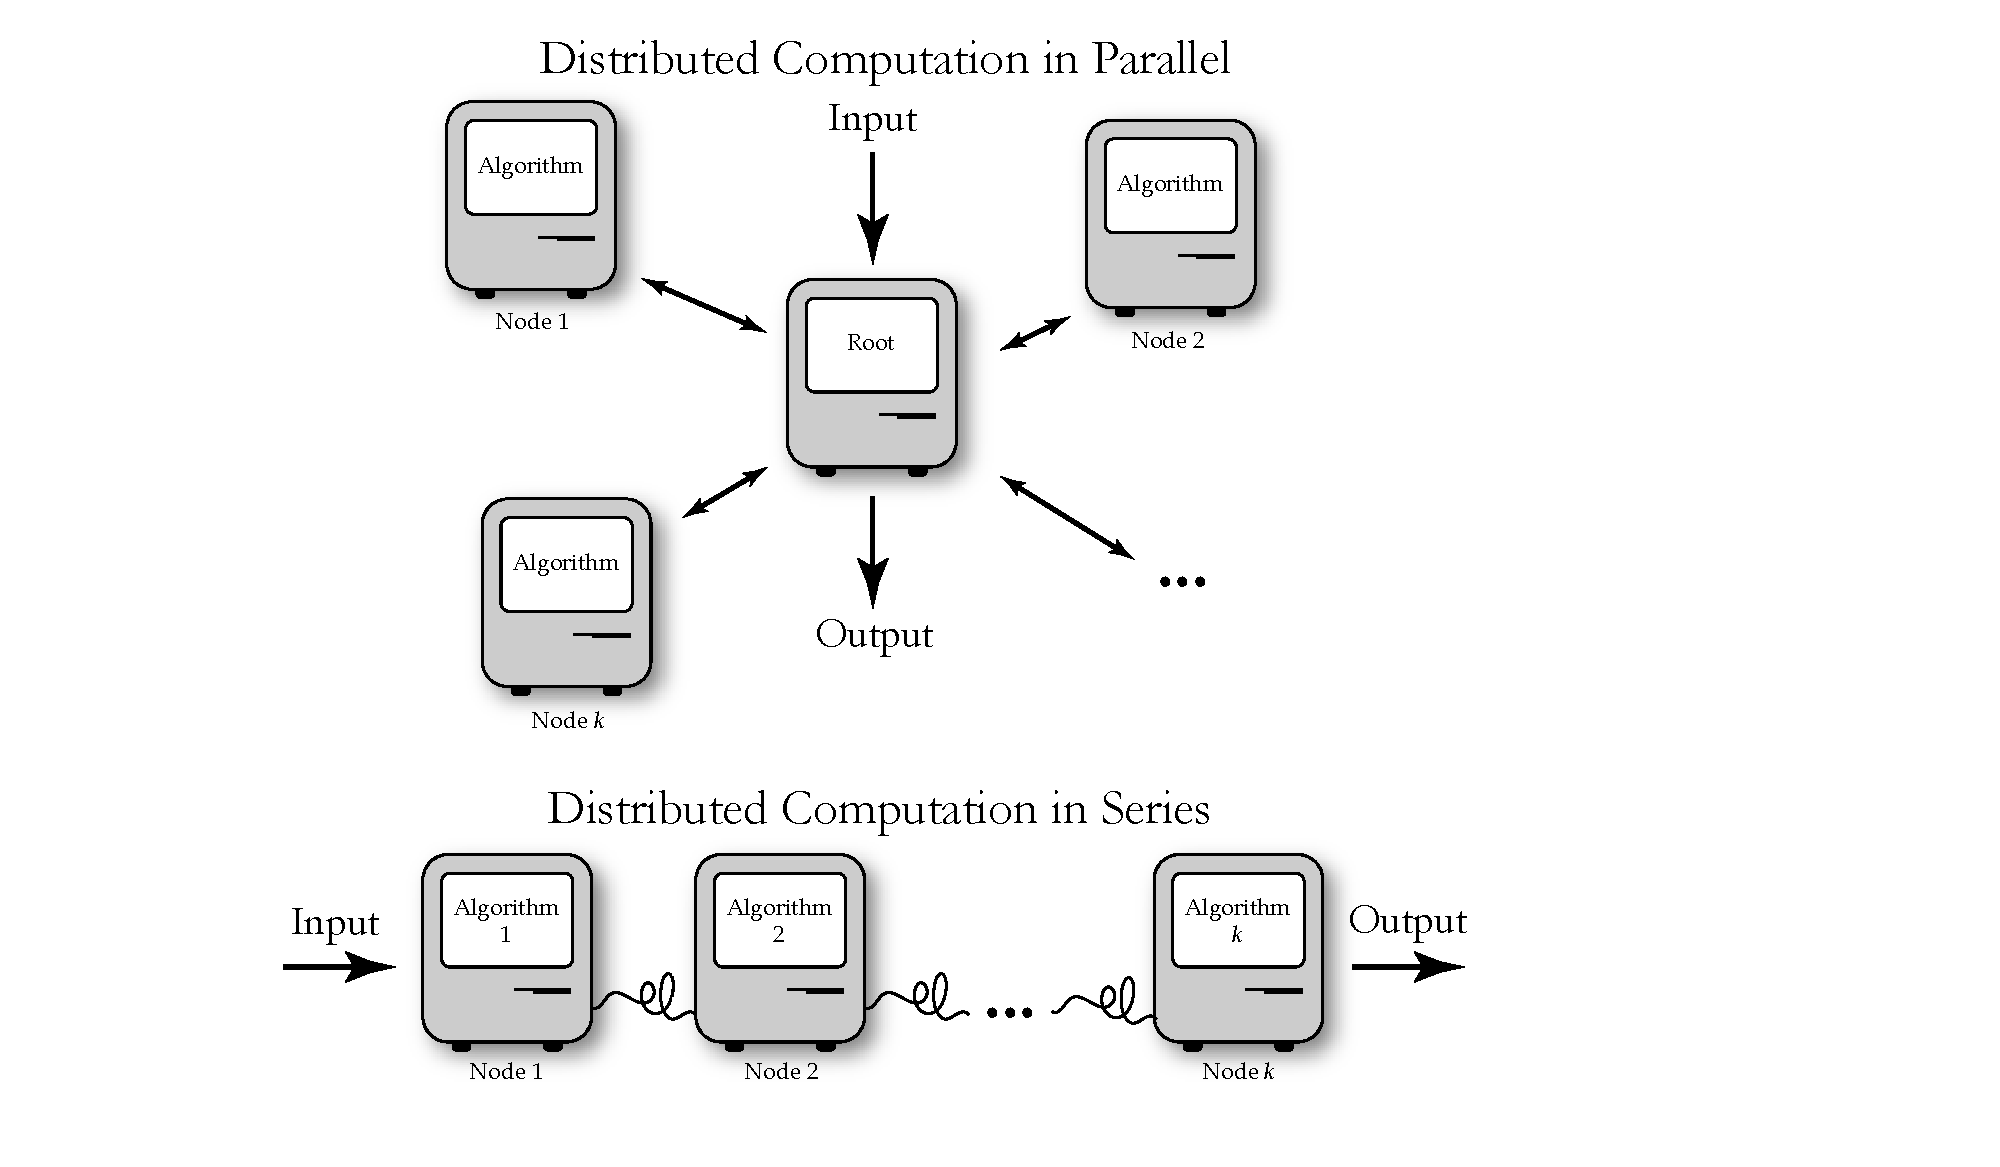
\includegraphics[clip=true, width=0.475\textwidth]{distributed}
\else
	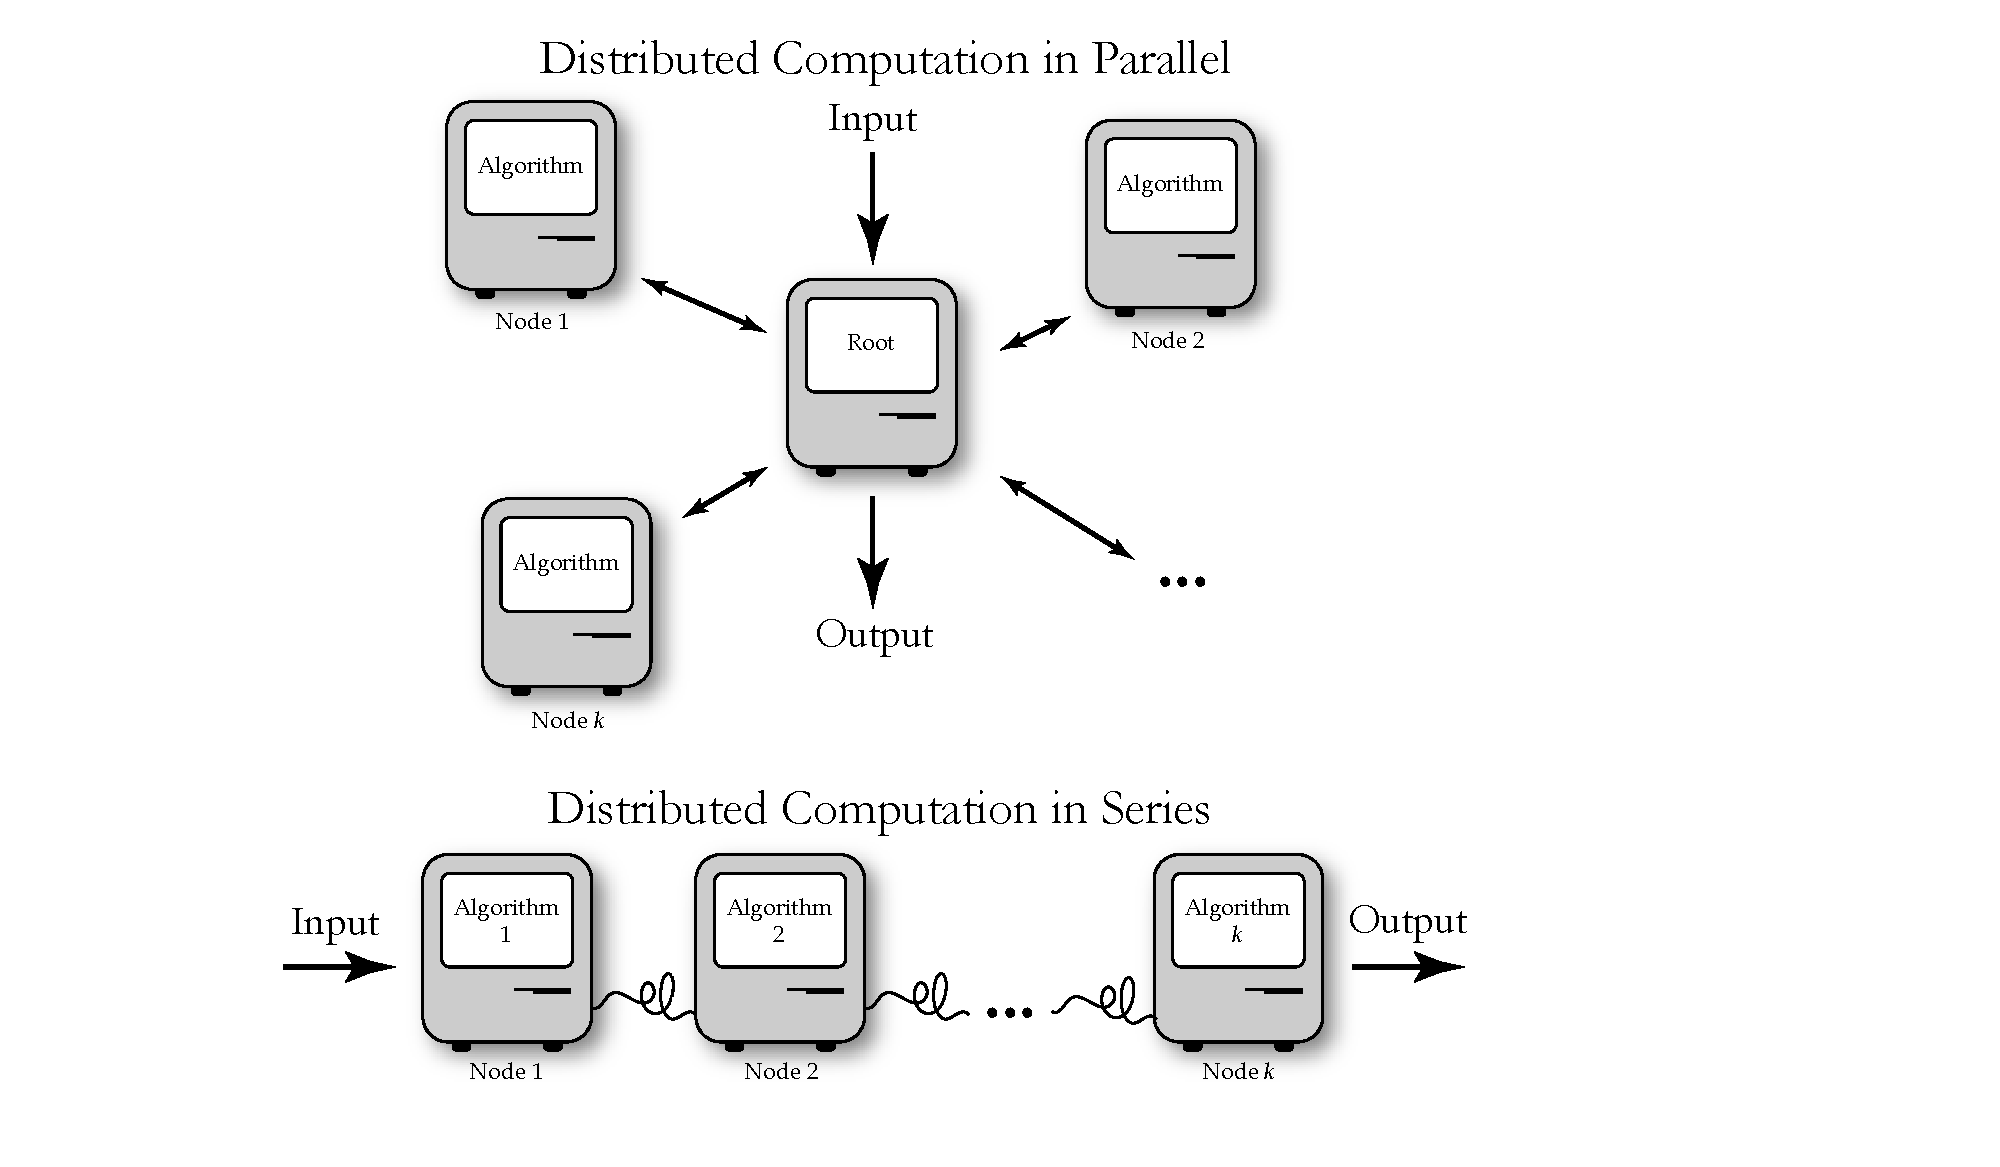
\includegraphics[clip=true, width=0.6\textwidth]{distributed}
\fi
\captionspacefig \caption{Models for distributed computation in parallel and in series. In parallel, a root node oversees the total computation, delegating tasks to child nodes, which process data independently of one another before being merged. In series the nodes sequentially process data in a pipeline of algorithmic stages.} \label{fig:distributed}
\end{figure}

Classical parallel processing typically involves a root node\index{Root node}, which delegates tasks to be performed in parallel by a number of child nodes, and the results returned to the root node, which potentially applies an algorithm to merge the set of results, before returning a final result to the client. Classical models such as Google's \textsc{MapReduce} protocol \cite{bib:MapReduce}\index{MapReduce} are built on this idea.

In classical computing, parallel processing is widely employed to shorten algorithmic runtimes. However, the increase in clock-cycles scales only linearly with the number of nodes in the network: $k$-fold parallelisation yields an \mbox{$\sim k$}-fold speedup. For time-critical applications, such a linear improvement may already be highly beneficial, albeit costly.

The alternate scenario is in-series distributed computation, in which a computation proceeds through a pipeline of different stages, potentially performed by different hosts. This model allows a complex algorithm comprising smaller subroutines, each of which may be proprietary with different owners, to be delegated across the network. The different stages may communicate classical and/or quantum data. As with the simple single-host model, if the different stages of the processing pipeline are sharing quantum data, distributed QEC will generally be necessary to protect the computation in transit. This necessarily introduces an (efficient) overhead in the number of physical qubits being communicated across the network, introducing additional bandwidth costs, which must be accommodated for in networking strategies.

\subsubsection{Quantum enhancement}

The attractive feature of quantum computing is the potentially exponential improvement in algorithmic performance of certain tasks over their classical counterparts as the size of the computer grows. This exponential relationship implies that computation in general no longer has a simple linear tradeoff as the number of participating nodes increases. In Sec.~\ref{sec:comp_sc_func} we quantify this via so-called \textit{computational scaling functions}\index{Computational!Scaling functions} and study its economic implications in detail.

But not every effort at distributed quantum computation will automatically exhibit the holy grail of exponential speedup. The architecture and algorithm to which it is applied must be thoughtfully designed to fully exploit the computers' quantum power. A simple adaptation of in-series or in-parallel computation may not achieve this. Rather, we must cunningly exploit quantum entanglement between nodes to perform truly distributed computation, in the sense that no instance of an algorithm is uniquely associated with any given node, but is rather represented collectively across all of them.

Let us assume that we have such a carefully constructed distributed platform. Let $t_c$ be the time required by a classical algorithm to solve a given problem, and $t_q$ the time required to solve the same problem using a quantum algorithm. In the case of algorithms exhibiting exponential quantum speedup, we will have,
\begin{align}
t_c = O(\exp (t_q)).
\end{align}
If we now increase the quantum processing power (i.e number of nodes or qubits) $k$-fold, the equivalent classical processing time is (in the best case),
\begin{align}
t_c' &= O(\exp (t_q k)) \nonumber \\
&= O(\exp (t_q)^{k}) \nonumber \\
&= O({t_c}^{k}).
\end{align}
Thus, $k$-fold quantum enhancement corresponds to a $k$th-order exponential enhancement in the equivalent classical processing time, which clearly scales much more favourably than the linear $k$-fold enhancement offered by classical parallelisation.

For this scaling to be possible, we expect that nodes will need to communicate via quantum rather than purely classical channels, so as to preserve inter-node entanglement and mediate non-local gates across nodes.

% Quantum MapReduce

\subsubsection{Quantum MapReduce}\index{Quantum MapReduce}\label{sec:quant_map_reduce}

Designing native distributed algorithms is not trivial, and architectural constraints may physically limit the allowed set of inter-node operations available to us. Are there any simple constructions that allow us to achieve this? We will propose an approach to parallelised quantum computation based on a direct quantum adaptation of the classical \textsc{MapReduce} protocol.

\textsc{MapReduce}, originally developed by Google\index{Google} for large-scale parallel processing, is simply an elegant formalism for parallelising classical computations. There are three stages to the protocol:
\begin{enumerate}
	\item \textsc{Map}: a root node\index{Root node} generates $k$ instances of an algorithm, each with different input data (or a different random seed).
	\item \textsc{Execute}: each of the $k$ instances are executed independently on the $k$ nodes in parallel.
	\item \textsc{Reduce}: all outputs are returned to the root node, collated and combined together according to some algorithm, yielding the final output of the computation.
\end{enumerate}

Perhaps the simplest illustrative example is to consider the execution of a Monte Carlo simulation\index{Monte-Carlo simulations}. Here we wish to execute a large number of instances of the same problem, each with a different random seed, and average the results to yield a statistical outcome. Here the \textsc{Map} algorithm simply delegates out $k$ copies of the same algorithm, assigning each node a different random seed\index{Random!Seed}, and the \textsc{Reduce} algorithm needs only average their outputs. Note that the \textsc{Map} and \textsc{Reduce} algorithms are relatively simple, with the nodes operating in parallel doing all the hardcore number crunching.

Taking this model, one might intuitively follow a similar approach for quantum computation, where we simply replace all the operations with unitary processes, and replace the communication links with quantum channels. Now we have a model as shown in Fig.~\ref{fig:quant_map_red}.

\begin{figure}
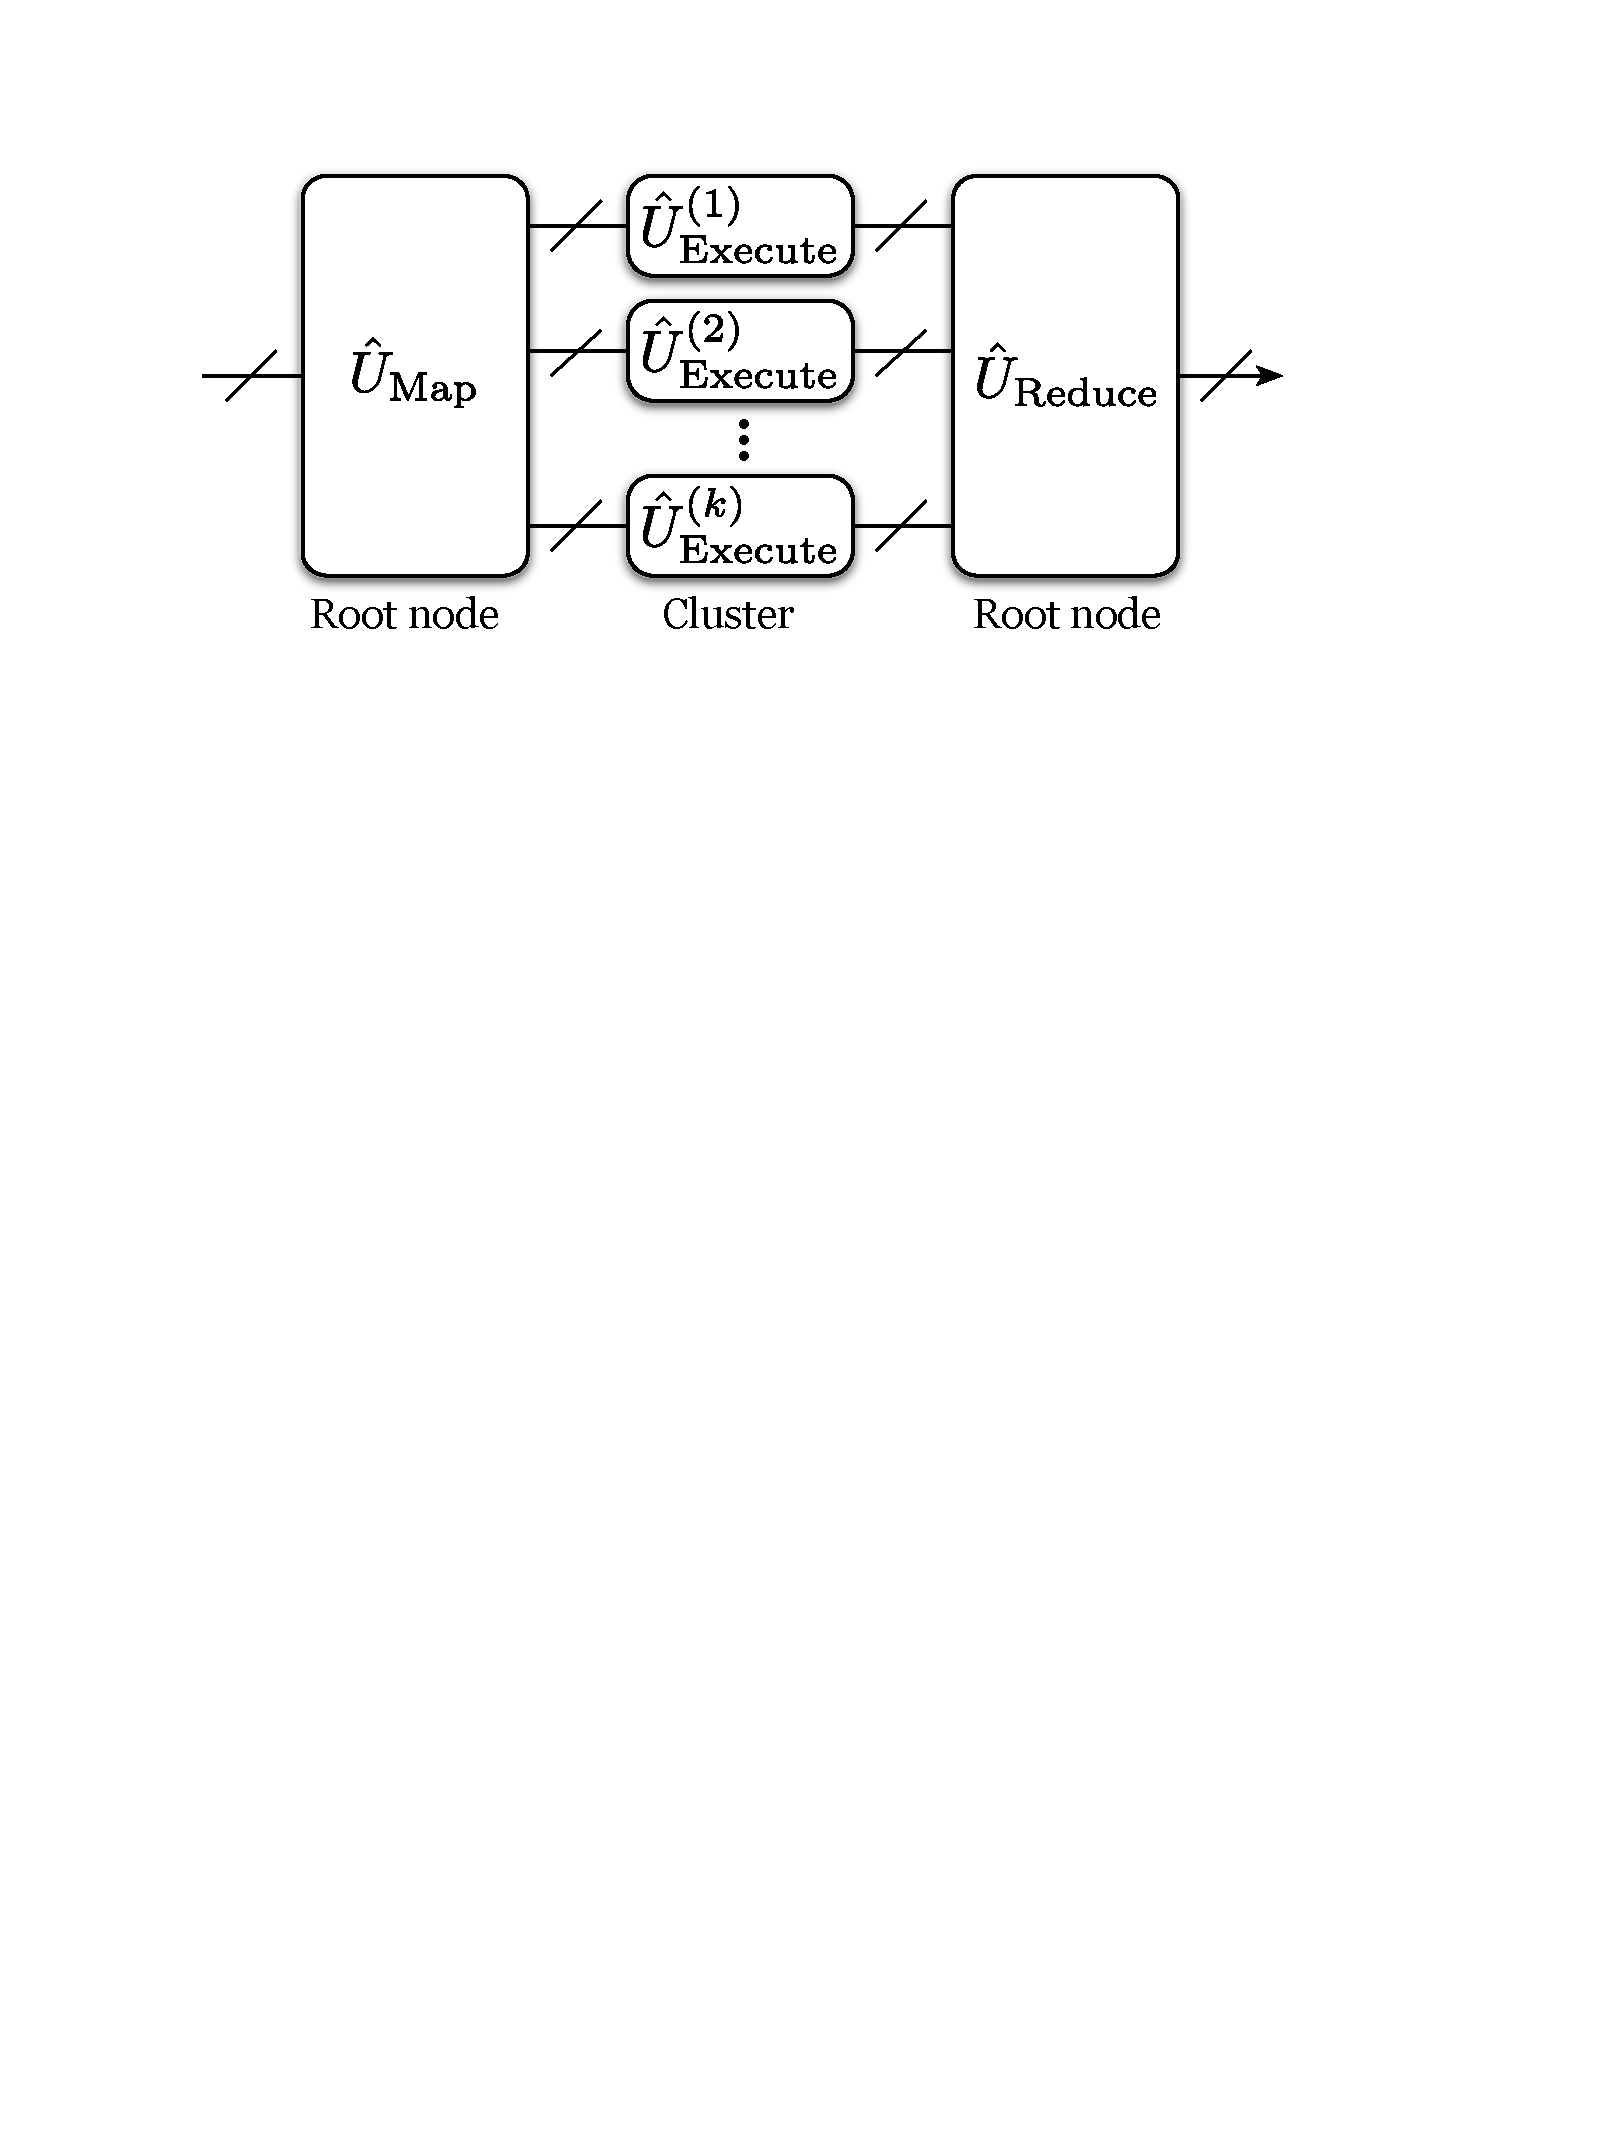
\includegraphics[clip=true, width=0.475\textwidth]{quantum_map_reduce}
\captionspacefig \caption{Structure of the quantum \textsc{MapReduce} protocol. All operations are unitary, and the \textsc{Map} and \textsc{Reduce} operations may be entangling in general. The \textsc{Execute} stage is separable into a tensor product of smaller \textsc{Execute} operations that are executed in parallel by the $k$ nodes.}\label{fig:quant_map_red}	
\end{figure}

The goal in this construction is to make the \textsc{Map} and \textsc{Reduce} operations be relatively very simple, e.g have low circuit depth, while the \textsc{Execute} operations are more challenging to implement. Note that the \textsc{Map} and \textsc{Reduce} operations are now unitary processes, rather than being, for example, simple classical dispatch and collate operations. This means that in general the \textsc{Map} operation will prepare entanglement between the \textsc{Execute} sub-computations, and \textsc{Reduce} might similarly implement non-separable entangling measurements to measure collective properties of the joint system.

This architecture is merely a direct mapping of classical \textsc{MapReduce} to the quantum setting. How might it be used? Consider quantum simulation\index{Quantum simulation}, where we aim to simulate a Hamiltonian of the form,
\begin{align}
\hat{H}_\mathrm{total} = \sum_i \hat{H}_i,	
\end{align}
where each of the $\hat{H}_i$ terms are local Hamiltonians acting on orthogonal Hilbert spaces. This implies that all terms commute,
\begin{align}
[\hat{H}_i,\hat{H}_j]=0,
\end{align}
and therefore the unitaries they generate,
\begin{align}
	\hat{U}_j=e^{-\frac{i\hat{H}_jt}{\hbar}},
\end{align}
have a separable tensor product structure,
\begin{align}
	\hat{U}_\mathrm{total}=\bigotimes_i \hat{U}_i.
\end{align}
This separability lends itself directly to the tensor product structure of the \textsc{Execute} unitaries. The \textsc{Map} operation could now be a stage for preparing entangled initial states (entangled across the different subsystems), and the \textsc{Reduce} operation might perform collective measurements or sampling.

% Distributed quantum search algorithm

\subsubsection{Distributed quantum search algorithm}\index{Distributed quantum search algorithm}

The Grover quantum search algorithm (Sec.~\ref{sec:quantum_search}) can be easily parallelised\index{Parallelisation} by partitioning the search space\index{Search space!Partitioning}, and allocating a different partition to each node.

Suppose we wish to search over the $N$-bit space $x$, to find a satisfying solution to some oracle\index{Oracles} function (e.g when solving an \textbf{NP}-complete problem\index{NP \& NP-complete}),
\begin{align}
x\,\, \mathrm{s.t.}\, f(x)=1.
\end{align}
Let there be $M$ nodes available for computation, where for simplicity we assume $M$ is a power of 2 (although the idea works generally for arbitrary $M$, albeit not as mathematically elegantly). We designate each of the nodes a $\log_2 M$-bit identification number\index{Identification numbers},
\begin{align}
	y=[0,M-1].
\end{align}
We now program each node to search over a smaller search space $x'$, which is \mbox{$N-\log_2 M$} bits in length, concatenated with the node's identification number to produce the full range of $x$. The input to each instance of the oracle is now,
\begin{align}
x = x'\frown y,
\end{align}
where `$\frown$' denotes binary string concatenation.

For example, with four nodes the 2-bit identification numbers are, 
\begin{align}
	y=\{00,01,10,11\}.
\end{align}
If the input search space is $N$-bits in length, then each of the nodes are assigned the search-space \mbox{$x'\frown y$}, where $x'$ is an \mbox{$N-2$}-bit number. Within each instance, the Grover search searches over only the reduced space $x'$, with $y$ a constant of the instance. Fig.~\ref{fig:distributed_search} illustrates the circuit schematic for the simple \mbox{$M=4$} example.

\begin{figure}[!htbp]
	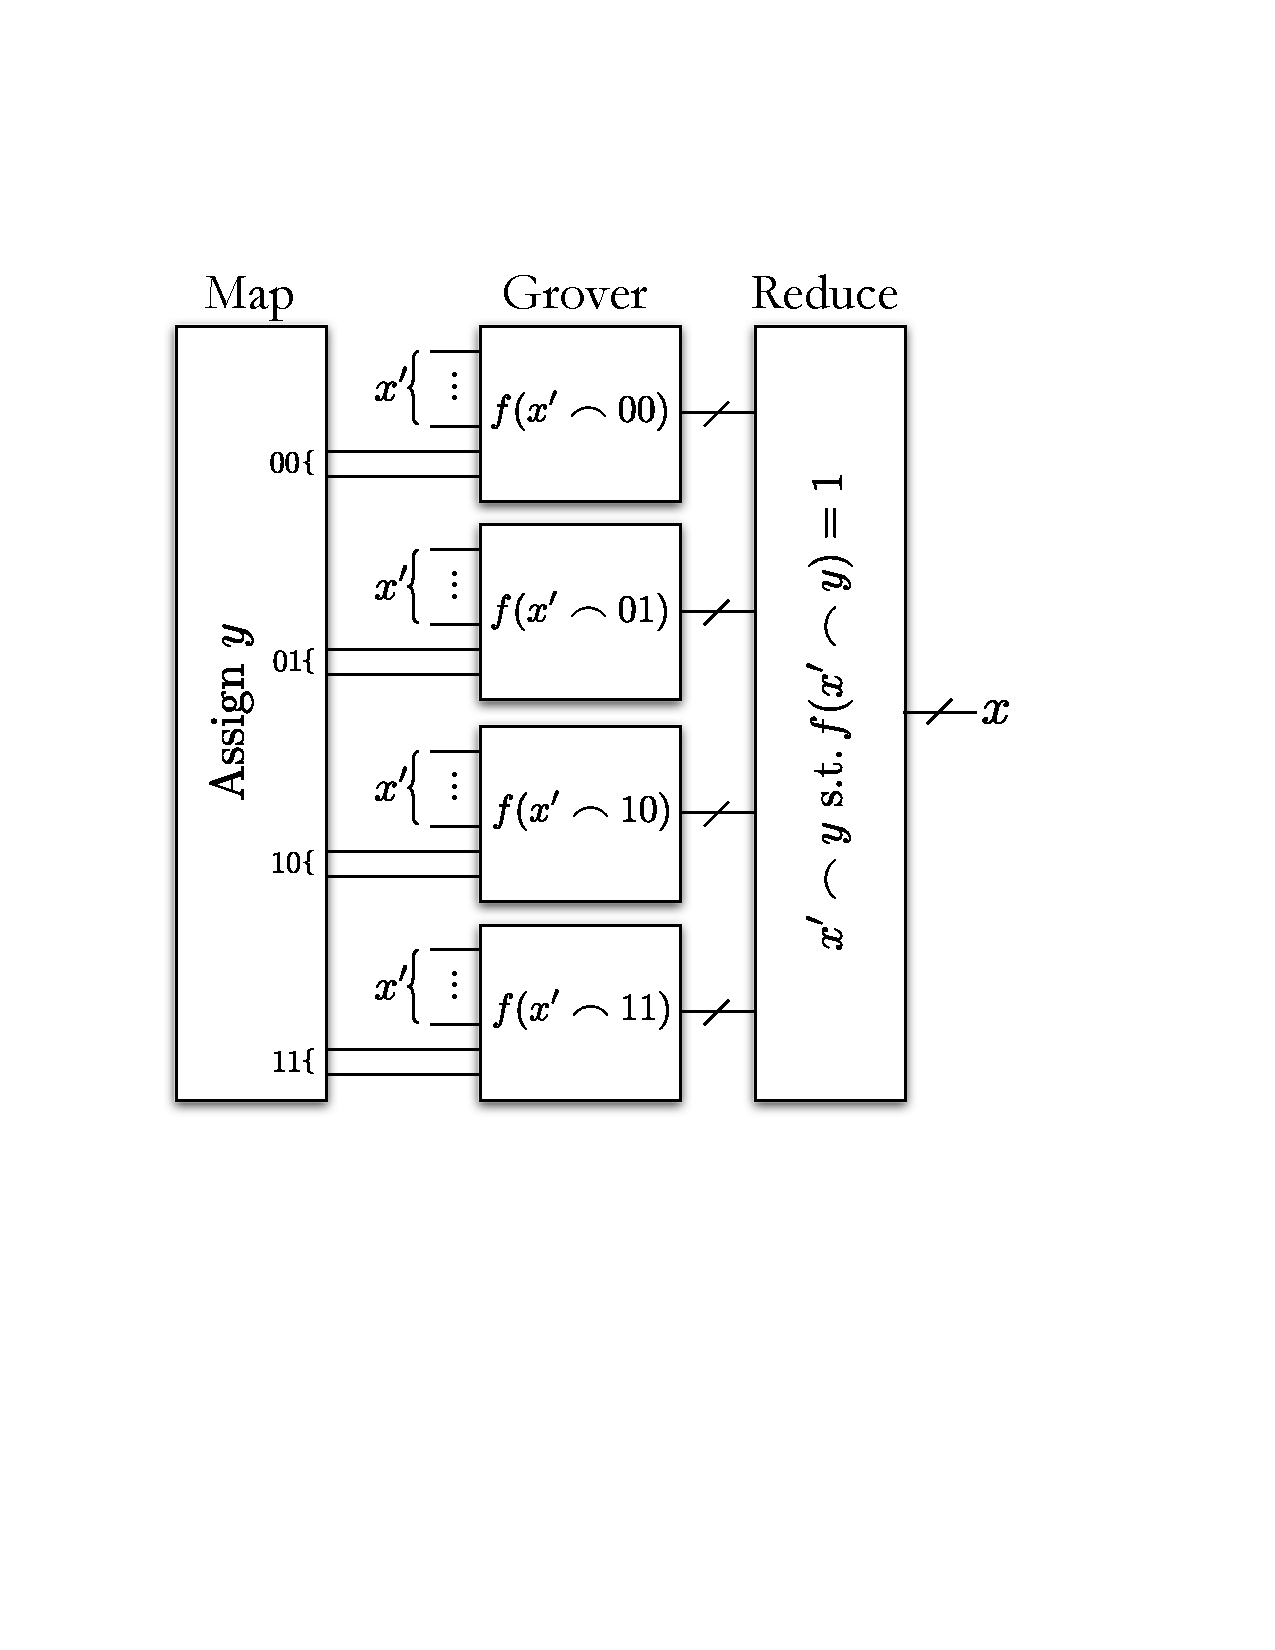
\includegraphics[clip=true, width=0.475\textwidth]{distributed_search}
	\captionspacefig \caption{Example of a quantum \textsc{MapReduce} protocol for implementing a distributed quantum search over four nodes. Each node performs a quantum search over the reduced space $x'$, concatenated with the identification number of the node, which recovers the full search-space $x$ across all the nodes collectively. This effectively partitions and allocates the search-space across the nodes, which implement their reduced searches in parallel. The net speedup provided by $M$ nodes operating in parallel scales as $O(\sqrt{M})$.}\label{fig:distributed_search}\index{Distributed quantum search algorithm}
\end{figure}

It can easily be seen that this approach is compatible with the general quantum \textsc{MapReduce} formalism (Sec.~\ref{sec:quant_map_reduce}), where the \textsc{Map} function assigns the partitions denoted by the node identification numbers $y$, the \textsc{Execute} functions implement the reduced searches associated with each instance, and the \textsc{Reduce} function collects satisfying arguments from the instances,
\begin{align}
	x'\,\, \mathrm{s.t.}\, f(x'\frown y)=1\,\,\forall\, y.
\end{align}

From the runtime of the Grover algorithm, it follows that the time required to solve the search problem on the initial full search-space is $O(\sqrt{2^N})$, whereas the time required in the parallelised implementation is only $O(\sqrt{2^{N-\log_2 M}})$. Thus, the need speedup is,
\begin{align}
	O\left(\frac{\sqrt{2^N}}{\sqrt{2^{N-\log_2 M}}}\right) = O(\sqrt{M}).
\end{align}

Evidently, the net computational speedup scales as a factor of the square root of the number of nodes in the parallelised implementation. Note that this approach does not exploit entanglement between nodes, and does not offer a `quantum' (i.e super-polynomial) speedup, since it's really just brute-force partitioning of a problem into smaller, quicker, bite-sized chunks that are attacked completely independently of one another, much like classical parallelisation.

To the contrary, unlike most quantum algorithms, whose power grows exponentially with the number of qubits (increasing returns\index{Increasing returns}), the distributed quantum search algorithm exhibits diminishing returns\index{Diminishing returns} with the degree of parallelisation -- the computational gain from adding one additional node to the network scales as,
\begin{align}
G=\sqrt{\frac{M+1}{M}},
\end{align}
shown in Fig.~\ref{fig:dist_quant_search}, which in the large $M$ limit asymptotes to,
\begin{align}
\lim_{M\to\infty} \sqrt{\frac{M+1}{M}} = 1.
\end{align}
That is, increasing the number of nodes from 1 to 2 has far greater net gain than increasing them from 100 to 101. In fact, asymptotically, the gain from adding an additional node vanishes in the limit of a high degree of parallelisation.

\begin{figure}[!htpb]
	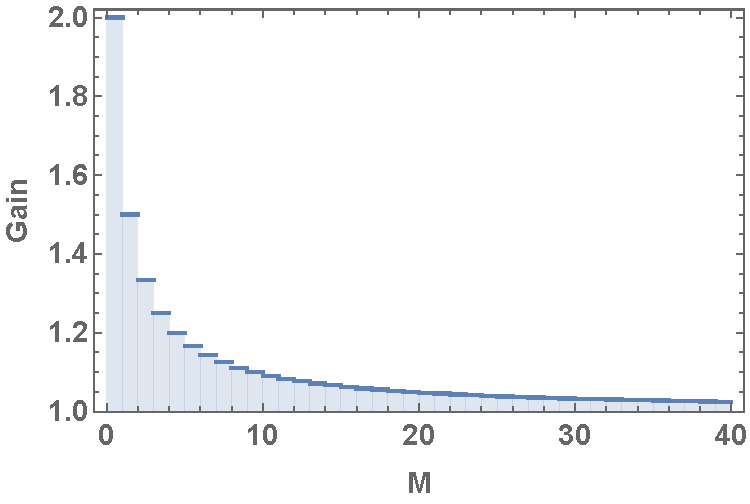
\includegraphics[clip=true, width=0.475\textwidth]{distributed_quantum_search}
	\captionspacefig \caption{Computational gain from adding a single extra node to a parallelised implementation of the quantum search algorithm. Asymptotically, the computational benefit vanishes.}\label{fig:dist_quant_search}
\end{figure}

For this reason, parallelised implementation of a quantum search is not an example of a distributed quantum computation which achieves exponential gain with the addition of new nodes (i.e qubits). Rather, for this specific application it's far more optimal to consolidate quantum resources into a single larger instance of a quantum search algorithm than using the quantum \textsc{MapReduce}\index{Quantum MapReduce} architecture to parallelise it.

% Distributed unitary error averaging

\subsubsection{Distributed unitary error averaging}\index{Unitary!Error averaging}\index{Distributed unitary error averaging}\label{sec:error_av_parallel}

In Sec.~\ref{sec:error_averaging} we introduced the unitary error averaging technique for minimising the errors associated with imperfect implementation of linear optics beamsplitter networks. This model is naturally of the form of \textsc{Quantum MapReduce}, where the \textsc{Map} and \textsc{Reduce} operations implement the fan-in and fan-out respectively, and the independent instances of the noisy unitary are executed in parallel on different nodes, as shown in Fig.~\ref{fig:error_av_map_reduce}.

\begin{figure}[!htbp]
	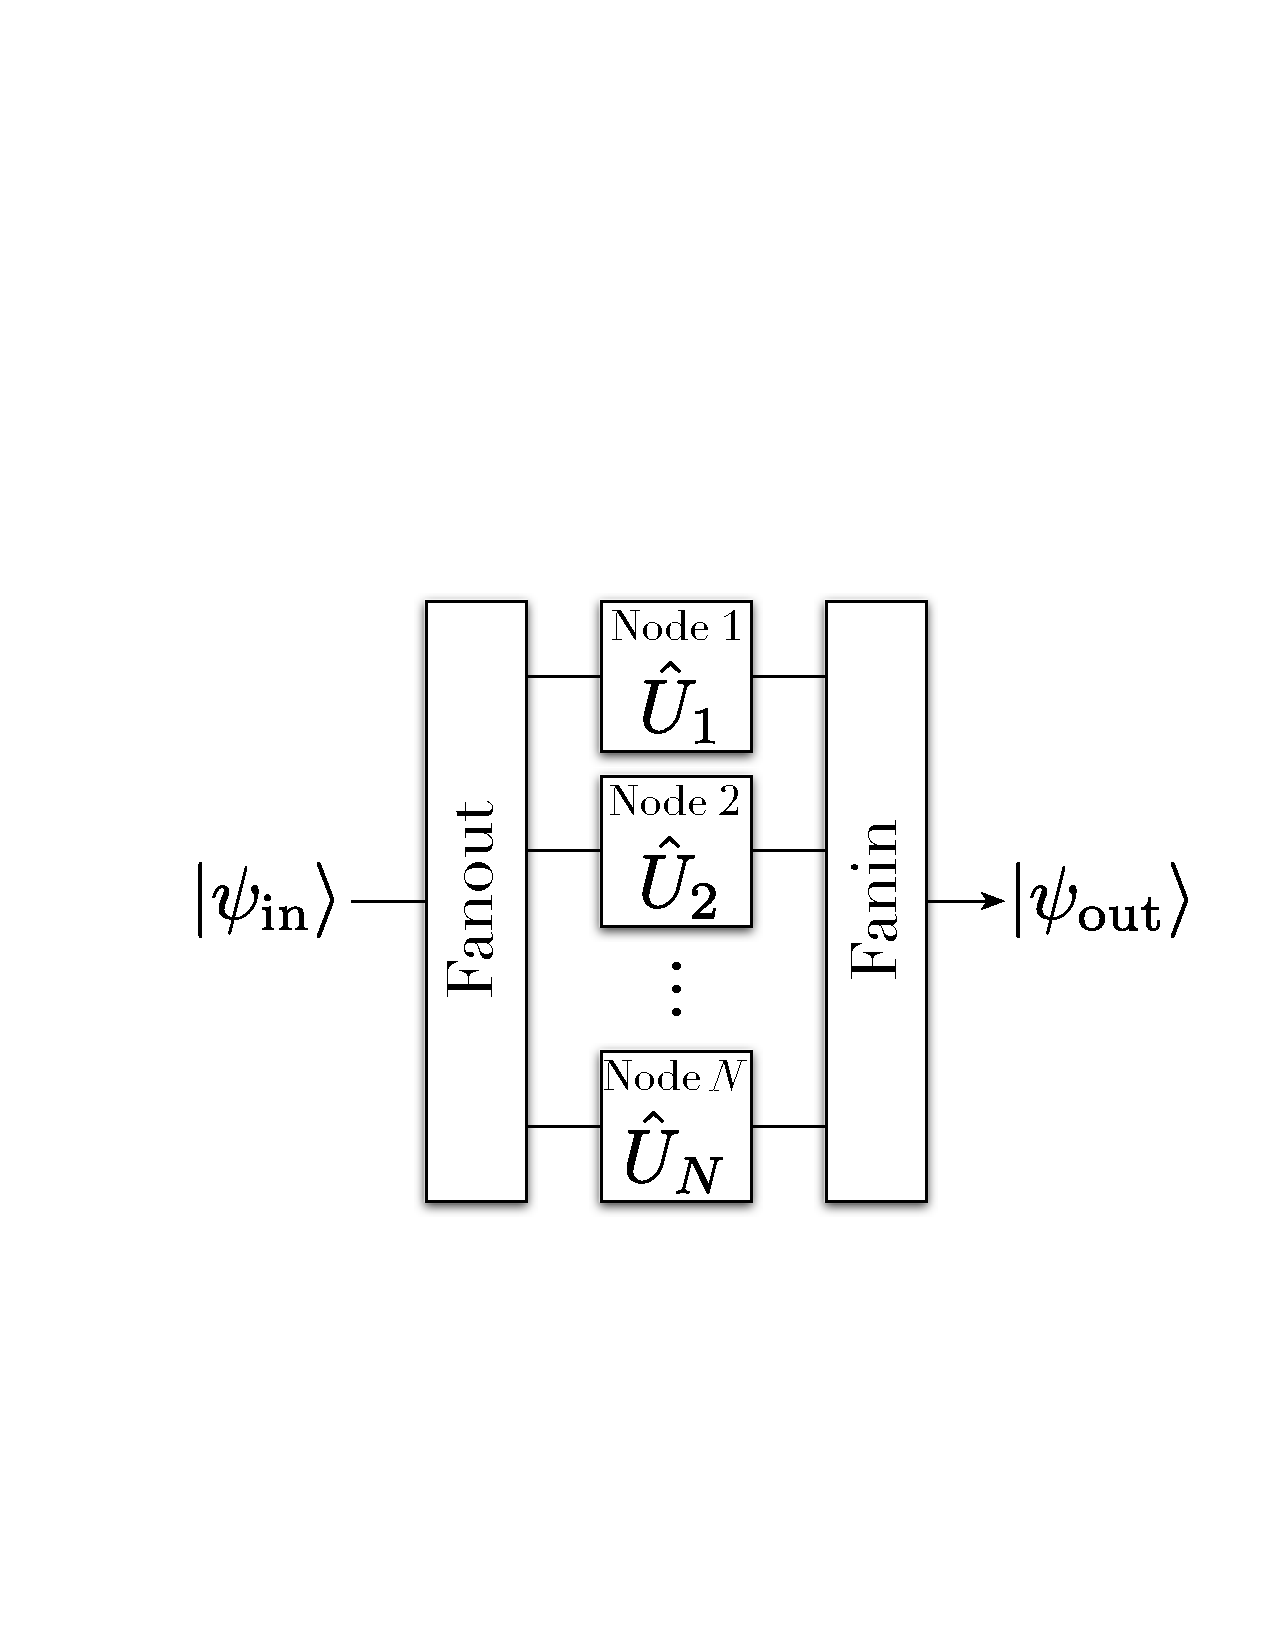
\includegraphics[clip=true, width=0.475\textwidth]{error_averaging_map_reduce}
	\captionspacefig \caption{Representing the unitary error averaging technique for error-correcting passive linear optics in parallelised form, consistent with the \textsc{Quantum MapReduce} structure.}\label{fig:error_av_map_reduce}
\end{figure}

Now the purpose of the parallelisation is not for computational gain, but rather for error minimisation. The more nodes involved in the parallelised execution, the smaller the final error rate.

\subsubsection{Delocalised computation}\index{Delocalised computation}

The cluster state (Sec.~\ref{sec:CSQC})\index{Cluster states}, topological code (Sec.~\ref{sec:surface_codes})\index{Topological!Codes} and quantum random walk (Sec.~\ref{sec:QW})\index{Quantum random walks} models for quantum computation may find themselves to be particularly well-suited to distributed implementation, since they naturally reside on graphs, whose nodes needn't be held locally by a single user, but could instead be shared across multiple hosts with the ability for graph nodes to intercommunicate. Then only classical communication is required to complete a computation and the quantum information is not localised to any particular node.

Additionally, the entangling gates which build cluster states all commute and may be implemented simultaneously in parallel. This enables a distributed cluster state to be constructed in a `patchwork' fashion, as shown in Fig.~\ref{fig:patchwork_cluster}. Now the computation is truly distributed in the sense that the computation resides collectively across the distributed cluster state, held by any number of users. No instance of an algorithm can be uniquely associated with any given node.

\begin{figure}[!htbp]
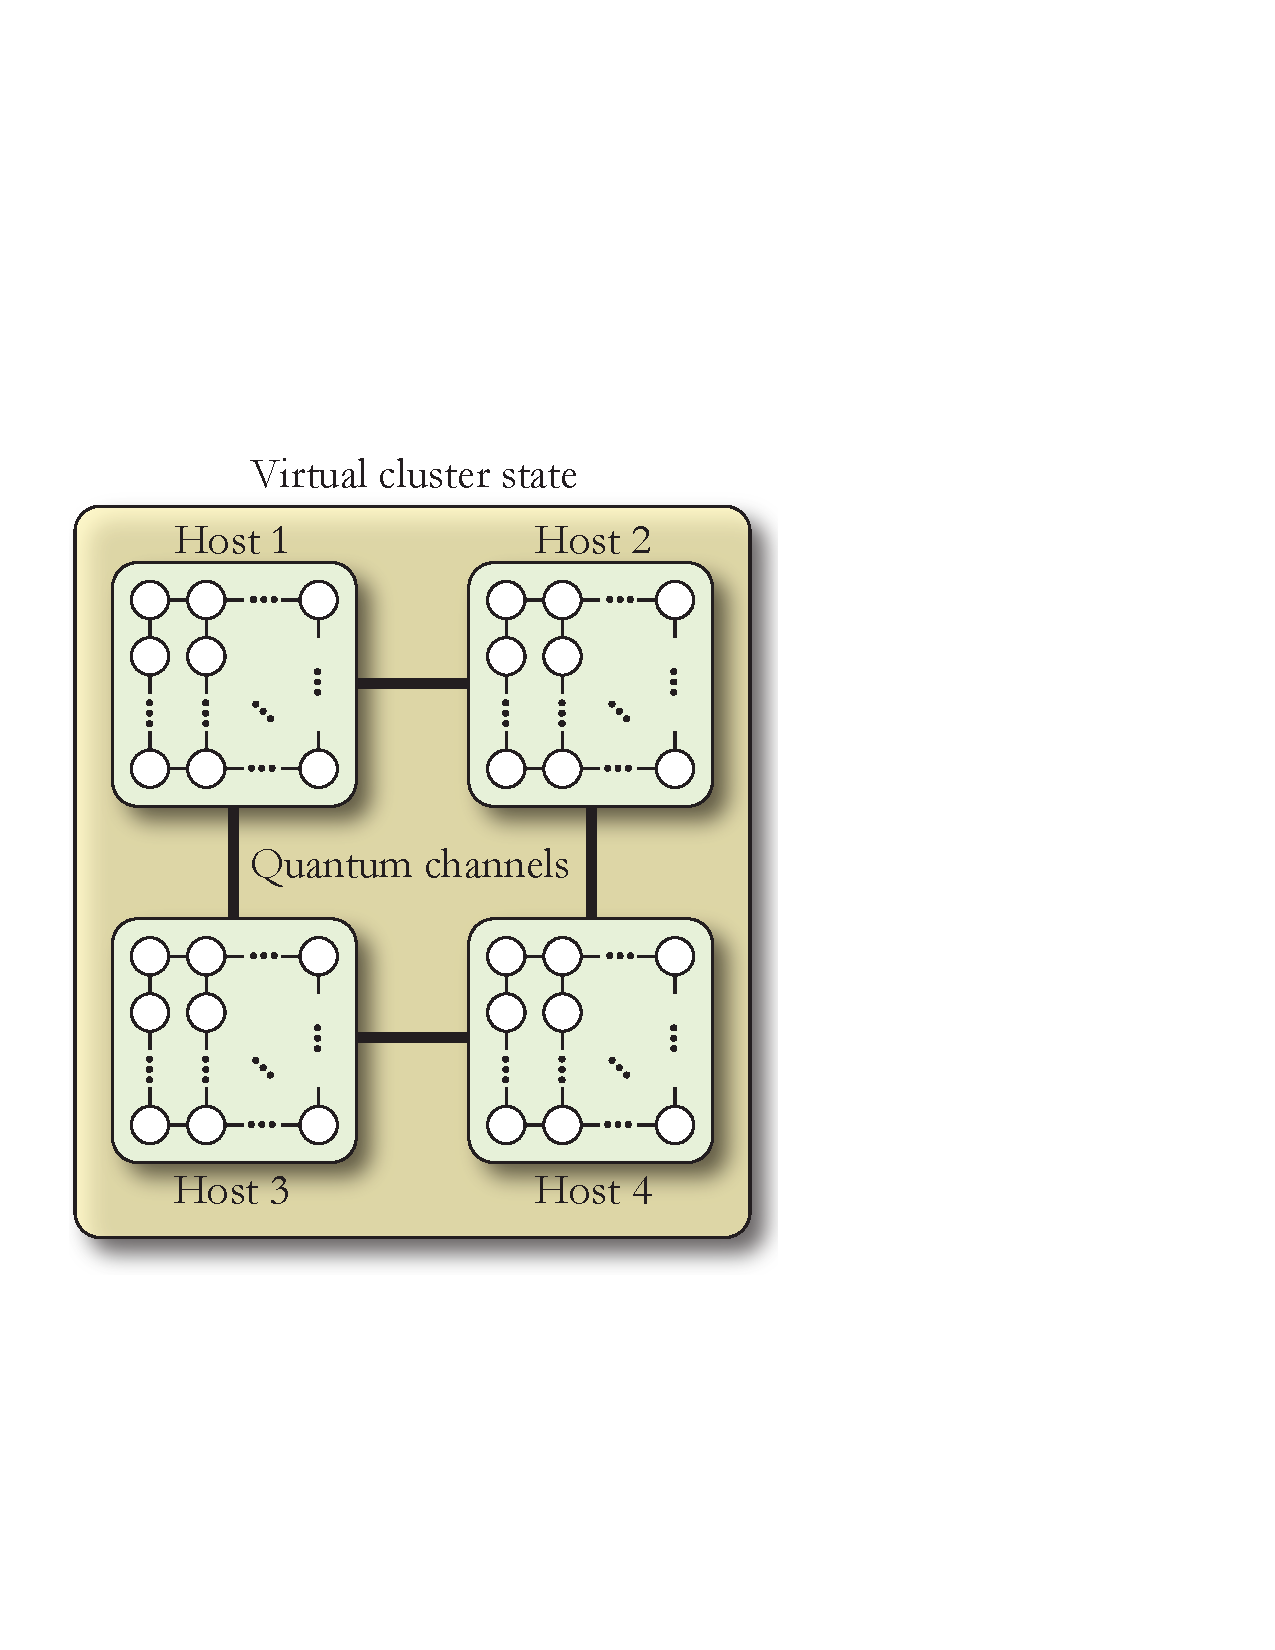
\includegraphics[clip=true, width=0.475\textwidth]{patchwork_cluster} 
\captionspacefig \caption{Approach for constructing distributed cluster states (or topological codes, or other graph states) across multiple nodes. The quantum channels allow neighbouring clusters in the topology to be fused together, constructing a large virtual cluster state for distributed computation. The nodes could be arbitrarily separated with optically-mediated interconnects to enable fusing nodes together.} \label{fig:patchwork_cluster}
\end{figure}

This approach overlaps with the modularised approach for quantum computation discussed in the upcoming Sec.~\ref{sec:module}, the difference being that in distributed cluster states the goal is to delocalise computations due to resource constraints, whereas for modularised computation the motivation is largely economical, driven by economy of scale.

%
% Delegated Quantum Computation
%

\subsection{Delegated quantum computation} 
\index{Delegated!Quantum computation}

Taking the notions of outsourced and distributed quantum computation to the logical extreme, we can envisage the situation where Alice has no quantum resources whatsoever (state preparation, evolution or measurement), but knows exactly what the processing pipeline should entail, and who on the network has the different required quantum resources. We refer to this as \textit{delegated quantum computation}, where the entire processing pipeline is outsourced to a series of hosts.

To illustrate this, let us consider a simple example -- cat state quantum computation (Sec.~\ref{sec:cat_enc}). There are three main elements to the protocol:
\begin{enumerate}
\item Cat state preparation.
\item Post-selected linear optics with feedforward.
\item Continuous-variable measurement.
\end{enumerate}

Each of these stages present their own technological challenges, sufficiently challenging that one might wish to outsource all three stages. However, suppose there is no single host on the network with the ability to perform all three, but rather there are three hosts ($B_1$, $B_2$ and $B_3$), each specialising in just one of those tasks. In this instance, it would be most resource savvy for the network to implement the pipeline,
\begin{align}
	A\to B_1\to B_2\to B_3\to A,
\end{align}
without going back and forth to Alice after each step,
\begin{align}
	A\to B_1\to A\to B_2 \to A\to B_3\to A.
\end{align}
In fact, it may not even be technologically possible to implement back-and-forth to Alice if she has no capacity for handling quantum resources (i.e the \mbox{$A\leftrightarrow B$} stages are purely classical). An example of such a pipeline is shown in Fig.~\ref{fig:delegated}.

\begin{figure}[!htbp]
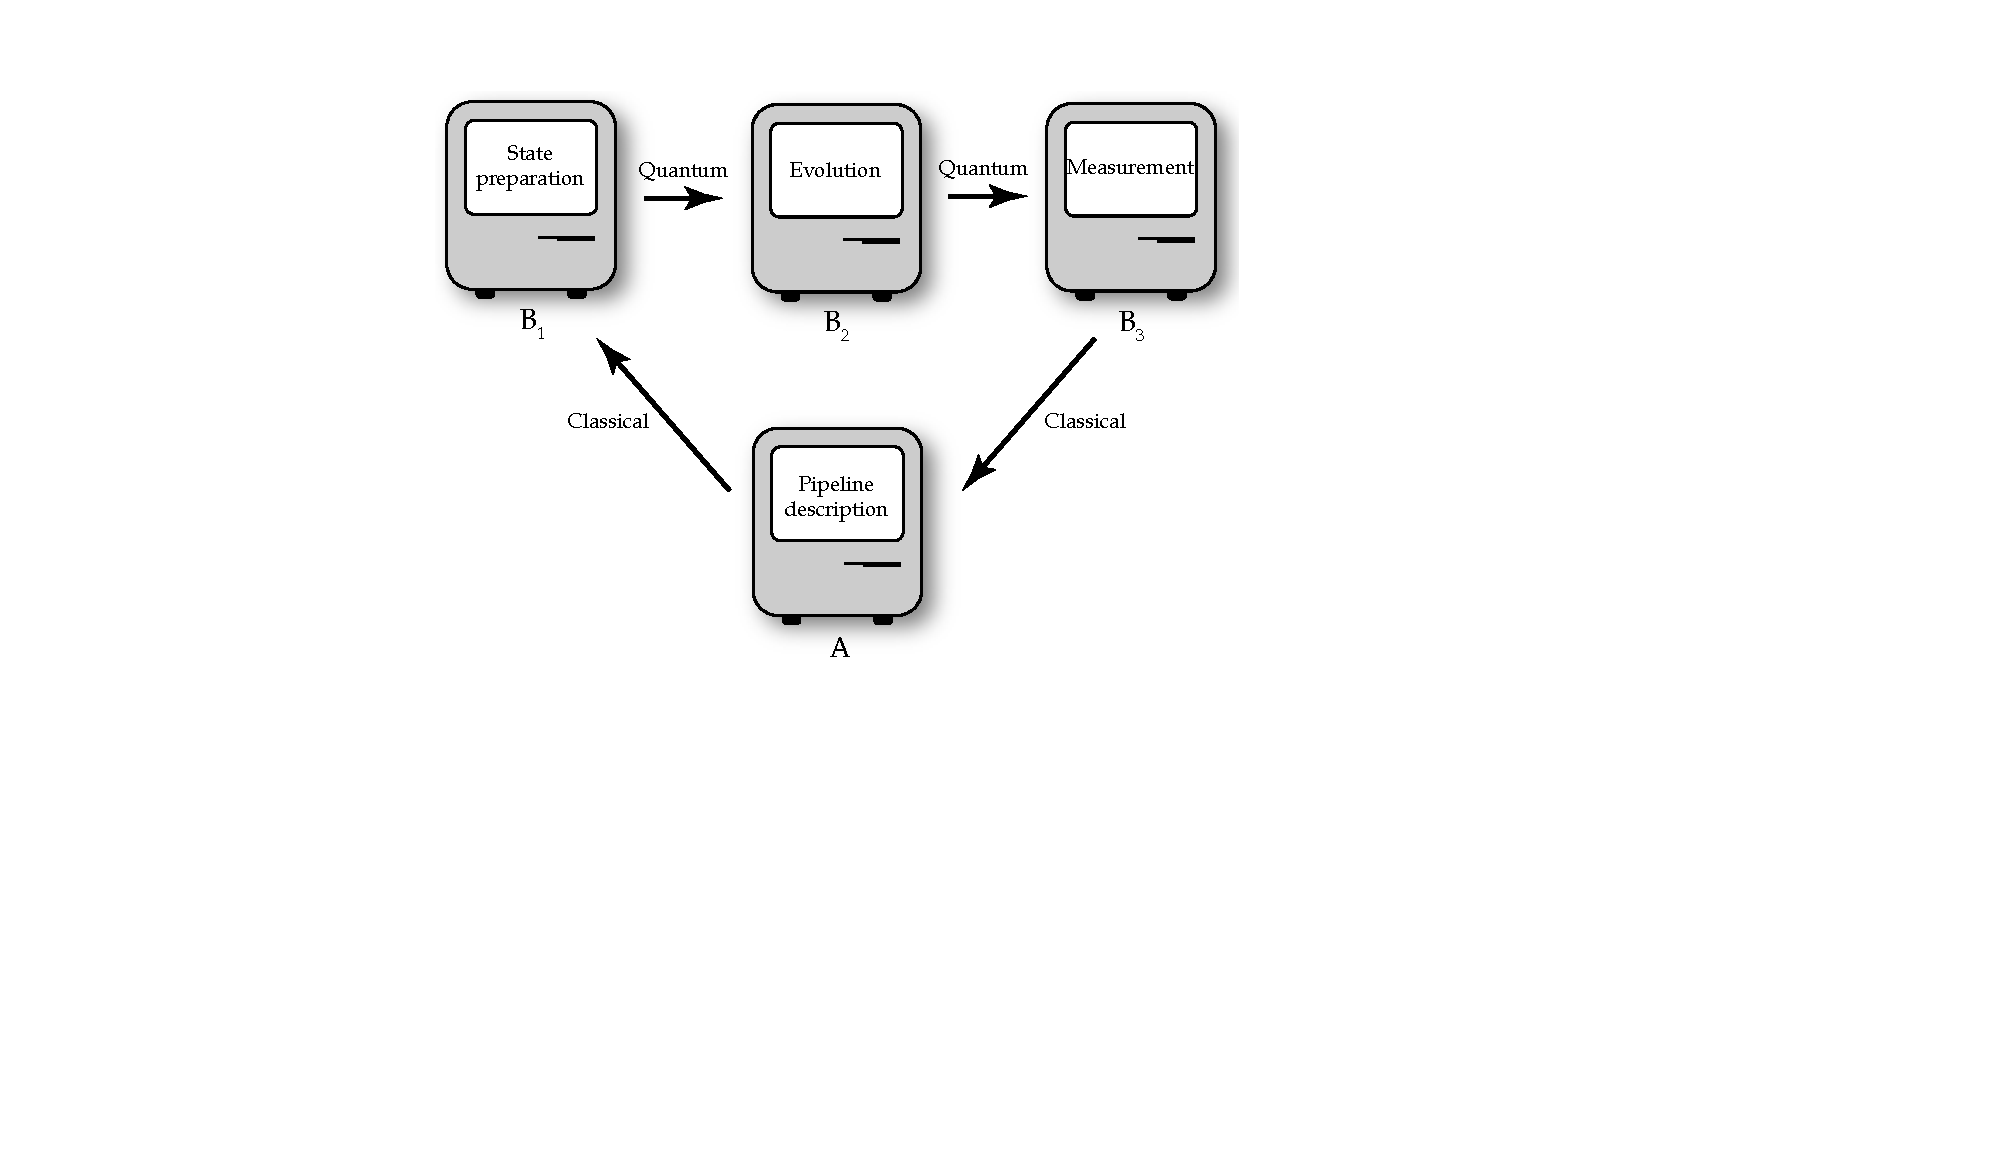
\includegraphics[clip=true, width=0.475\textwidth]{delegated}
\captionspacefig \caption{Delegated quantum computation, where each of the three computational stages (state preparation, evolution and measurement) are outsourced to the cloud without intermittent interaction with the client, $A$. $A$ provides only a classical description of the processing pipeline to be implemented, each stage of which is delegated to a server specialised in that particular task. Thus, the total processing pipeline takes the form \mbox{$A\to B_1\to B_2\to B_3\to A$}, where \mbox{$A\to B_1$} and \mbox{$B_3\to A$} are classical, and \mbox{$B_1\to B_2$} and \mbox{$B_2\to B_3$} are quantum channels.} \label{fig:delegated}
\end{figure}

This can be achieved by adding a \textsc{Pipeline} field to the packet header prepared by Alice -- a FIFO queue describing the entire processing pipeline that Alice's packet (which initially contains only classical data) ought to follow through the network. Following completion of each stage of the pipeline we pop the stack and transmit the packet to the next specified host. Only at the very completion of the protocol is a packet (containing only classical data) returned to Alice.

Another good case study is quantum metrology using NOON states (Secs.~\ref{sec:NOON} \& \ref{sec:metrology}) for achieving Heisenberg limited precision. Preparing NOON states is extremely challenging, and additionally Alice may not possess the unknown phase to be measured, but rather wishes a NOON state, prepared by $B_1$, to be provided to a third party, $B_2$, who applies the unknown phase, and passes the resulting state to $B_3$, who implements the required high-efficiency parity measurements required to complete the protocol. In this case, the pipeline would take the same form as above, again with no back-and-forth communication to Alice.

Such delegated protocols will be very useful in quantum networks, where different hosts specialise in different tasks (which may be the most economically efficient model), but poor old Alice specialises in none of them, despite knowing exactly what needs to be done. This would allow an aspiring undergraduate student, who is poor (aren't they all?), to sit in his bedroom at his classical PC, and implement entire distributed quantum information processing protocols in the cloud, with no quantum resources or interactions whatsoever.

%
% Modularised Quantum Computation
%

\subsection{Modularised quantum computation} \label{sec:module} \index{Modularised quantum computation}

How does one build a large-scale quantum computer, given the extremely daunting technological requirements and high costs? In any industry, economies of scale allow the mass production, and rapid reduction in price of technology. To achieve this, we must find a way to make quantum technologies commodity items, which avoid all the hassle of customised cutting-edge labs. What we really desire is production-line `Lego for Adults{\texttrademark}', allowing ad hoc connection of \textit{modules}, which implement small subsections of a larger computation \cite{bib:FowlerPrivate}.

We envisage that physically, a module is a black box with optical interconnects, that may be interconnected to form an arbitrary topology, yielding a physical platform as shown in Fig.~\ref{fig:modules_physical}. The user remains oblivious to the inner workings of the modules. The modules could all be identical, just patched together differently, paving the way for their mass production, and an associated quantum equivalent of Moore's Law, allowing them to become off-the-shelf commodity items over time. Then the cost of a quantum computer would simply scale linearly with its number of qubits.

\begin{figure}[!htbp]
	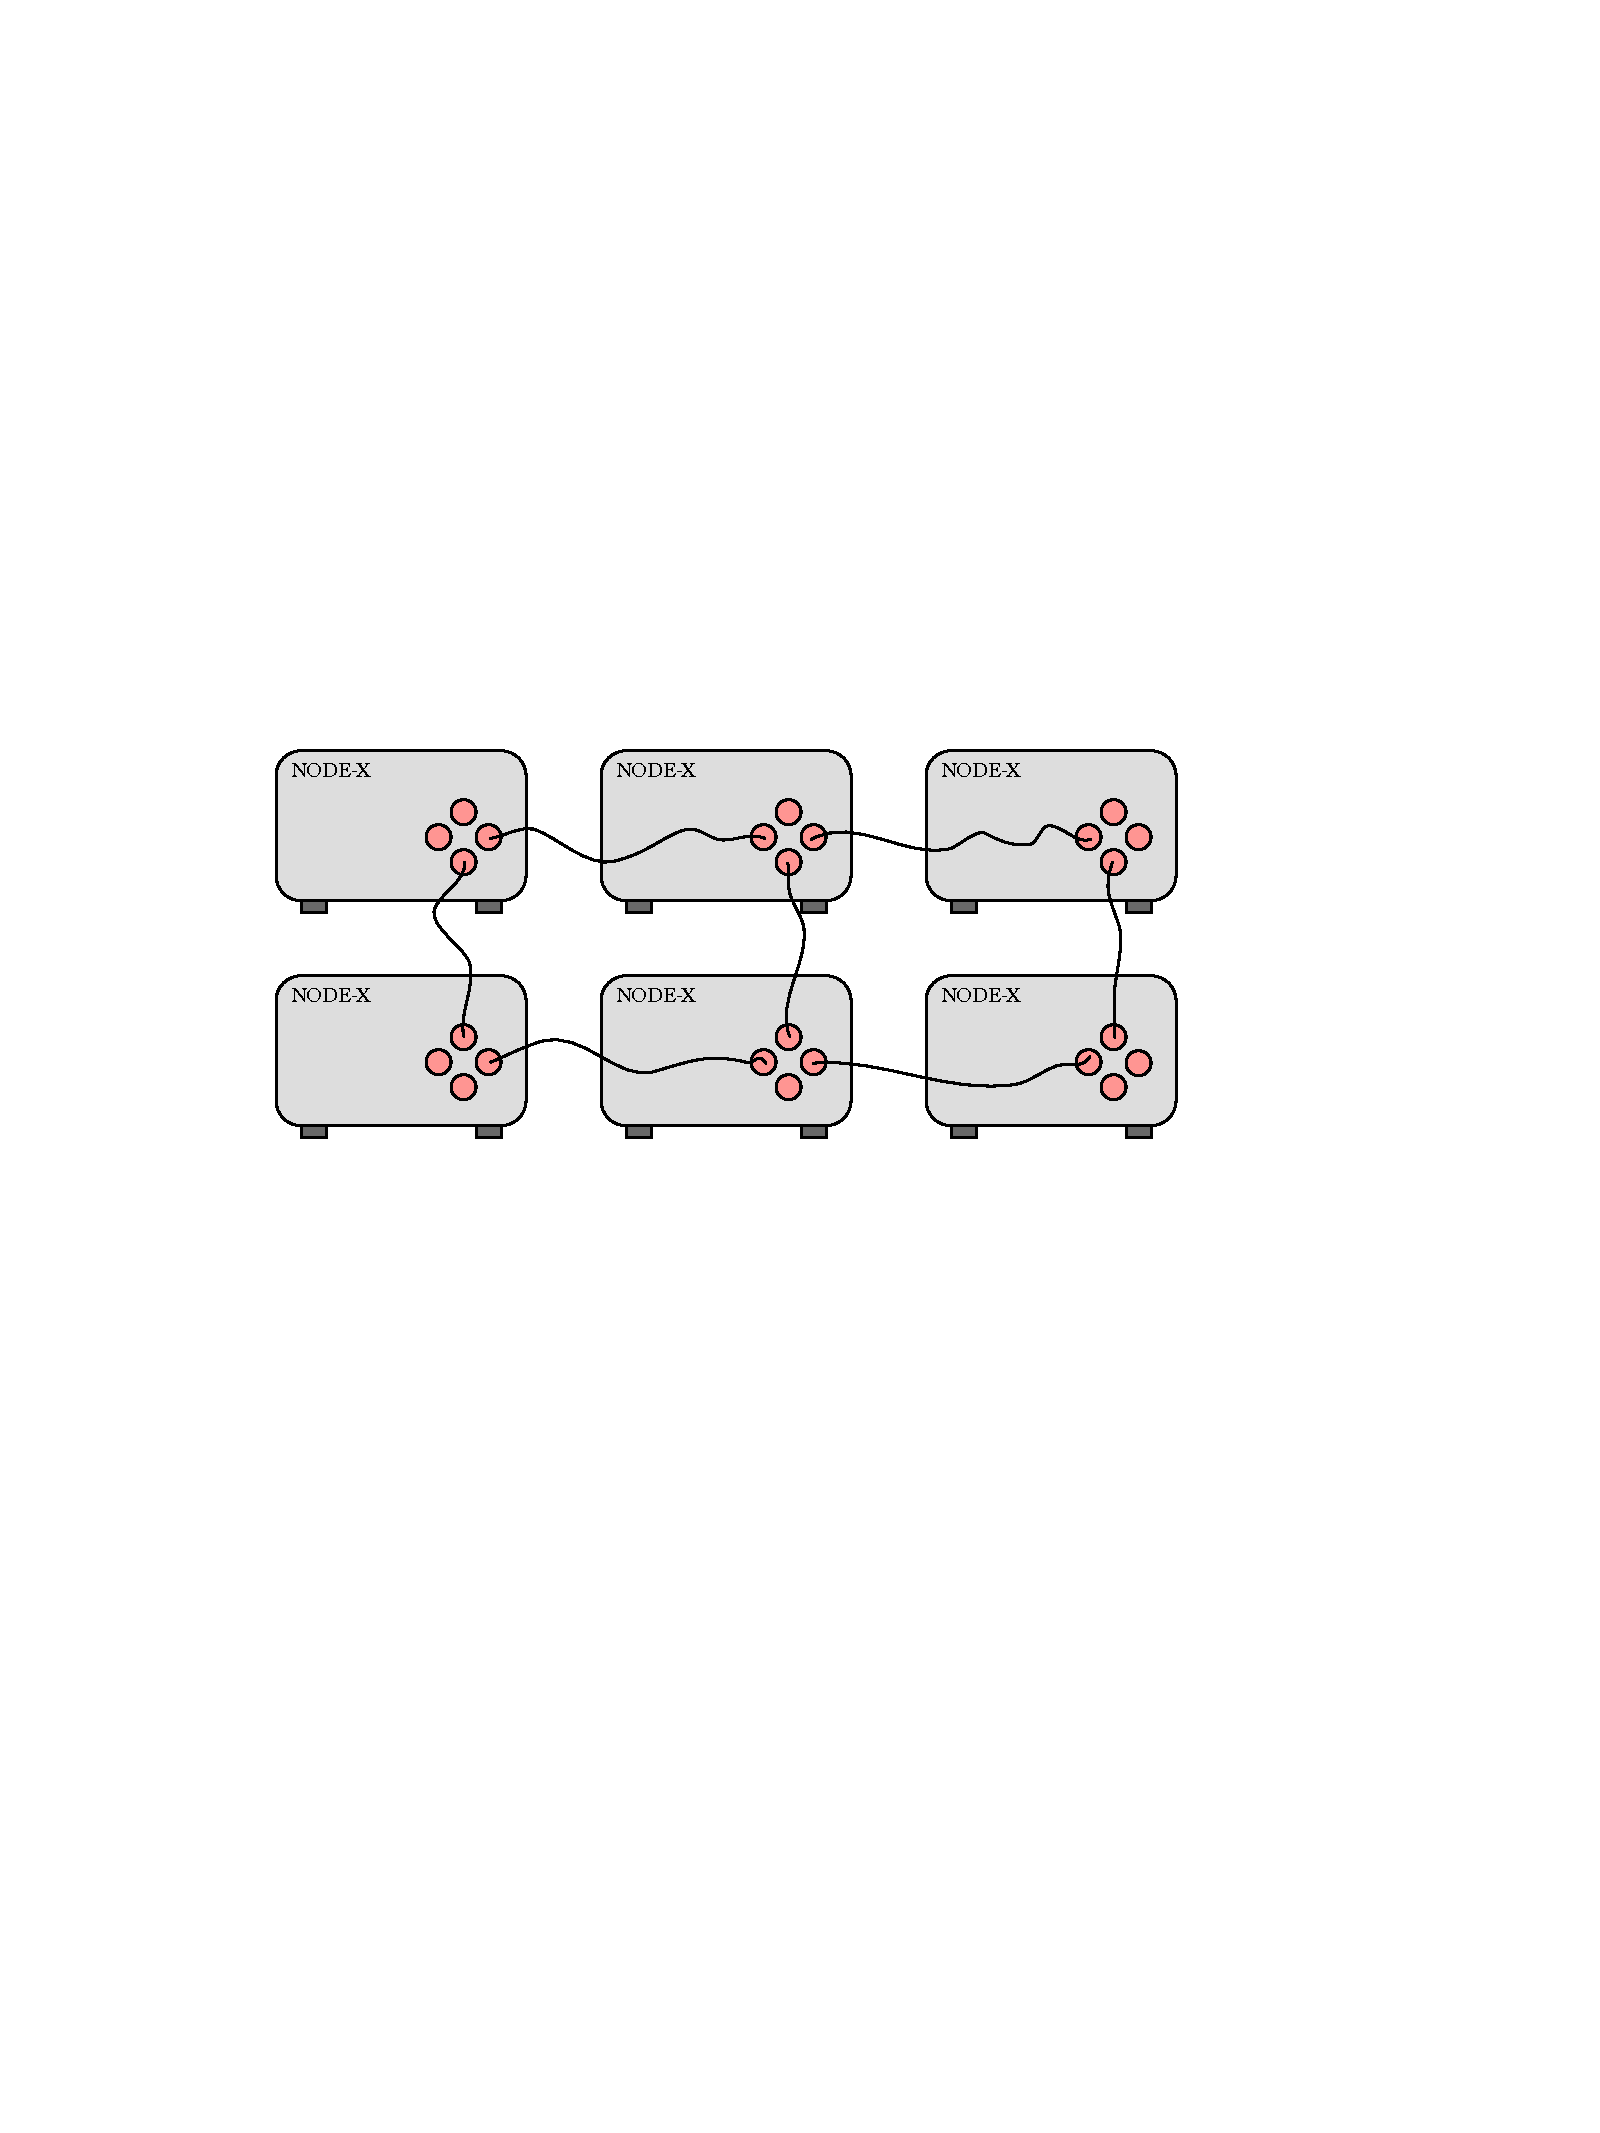
\includegraphics[clip=true, width=0.475\textwidth]{modules_physical}
	\captionspacefig \caption{A possible physical realisation of commercially produced quantum modules\index{Node-X}, forming a \mbox{$2\times 3$} patchwork of cluster states. Each hosts a relatively small number of qubits. The nodes each have four optical interconnects, which are used to connect the modules via optical fibre. Entangling operations performed on photons shared via the interconnects create inter-module entanglement links, yielding a distributed virtual quantum computer with far more qubits. The computation is truly distributed and cooperative, in the sense that the entire computation is non-local, instead being collectively distributed across all the nodes, which coordinate their local operations via only classical communication. An alternate implementation is to replace the inter-node quantum links with Bell pair distributers. Then entanglement swapping can be employed to swap the entanglement into a link between nodes.}\label{fig:modules_physical}
\end{figure}

The modules forming a particular computation could either be all owned by a single well-resourced operator, or alternately might be shared across multiple hosts, who network them remotely using EOs\index{Entangling operations} between emitted photons.

In Sec.~\ref{sec:dist_QC} we introduced the notion of distributed quantum computation. There the motivation was to enable a computation to be distributed across multiple servers, which either parallelise computation or process it as a pipeline in series.

An alternate direction, for economic reasons, is that it is unviable for a single server to host an entire computation. Rather, hosts will have limited capability, and performing large-scale computations will require employing a potentially large number of hosts cooperating and sharing resources with one another\footnote{Even some present-day massive-scale data processing and storage protocols are implemented virtually across multiple large-scale data-centres, which, for example, automatically handle geographically decentralised data redundancy and processing. Google and Amazon, for example, provide cloud services for this purpose, employed both internally, and licensed out to third parties, and the Apache Cassandra\index{Apache Cassandra project} project provides an open-source equivalent. The key is for the underlying protocol to abstract this away from the user, such that they interface with the data as though it were a local asset.}. This can be regarded as the most general incarnation of distributed computation.

This is not the same motivation as for in-series computation, where different servers in the pipeline have different proprietary algorithms as subroutines of a larger computation. And it also differs from in-parallel computation, where multiple servers implement the same algorithm on different data, which is subsequently merged by a root node, as per, for example, a \textsc{MapReduce}-style protocol.

Instead, the motivation is one of economics. First, individual servers will have finite resources, but there may be many of them, which can be networked to cooperatively implement a larger algorithm virtually. Second, because the modules in the architecture are identical and lend themselves to mass production, one can expect more favourable economics than that offered by a provider who sells full-fledged, customised quantum computers, which do not lend themselves to the same level of mass production.

The concept of this model is best explained using the optical cluster state formalism (Sec.~\ref{sec:CSQC}), which lends itself naturally to this approach. A rectangular lattice graph is sufficient for universal quantum computation, even if the cluster state graph is not local (but classical communication between nodes is allowed).

Let us first assume that we wish to construct a cluster state with $n_\mathrm{logical}$ logical qubits. We additionally allow each logical qubit to be the root node of a graph with a $+$-structure, where each branch comprises a chain of $n_\mathrm{ancilla}$ ancillary physical qubits. These are sometimes referred to as \textit{micro-clusters} \cite{bib:Nielsen04}\index{Micro-cluster states}. A single micro-cluster collectively forms a single \textit{module} in the topology. Our goal is to fuse modules via nearest neighbour entanglement to build up the desired distributed cluster state.

\if 2\pubmode
\begin{figure}[!htbp]
	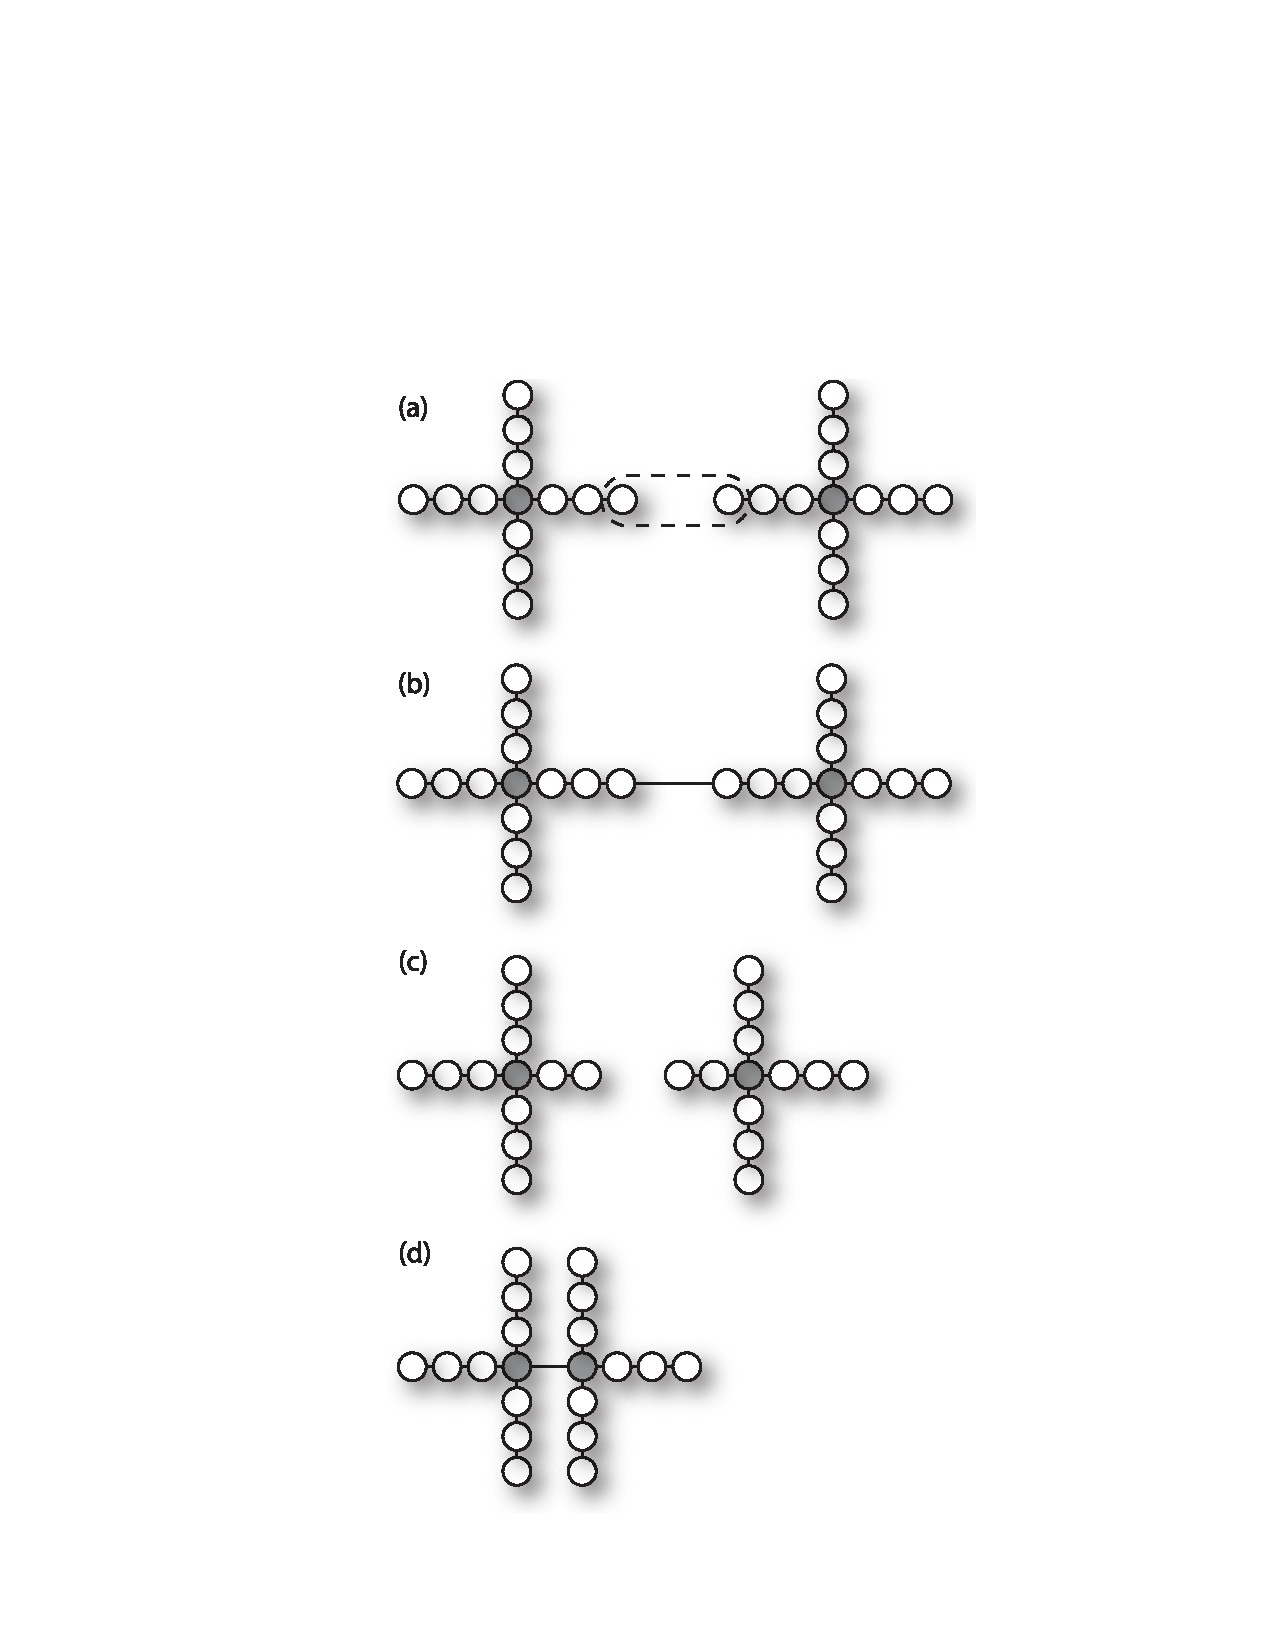
\includegraphics[clip=true, width=0.4\textwidth]{cluster_ident_long}
	\captionspacefig \caption{Several cluster state identities for modularised quantum computation. (a) Two cluster states with a $+$-topology are fused together using an EO (dashed). (b) Upon success, an edge is created between the respective qubits. (c) Upon failure, both qubits are effectively measured in the $\hat{Z}$ basis, thereby removing them, and any associated edges, from the graph. (d) Following a successful EO, the unwanted ancillary qubits may be eliminated using measurements in the $\hat{Y}$ basis, creating edges between their neighbours. If the grey qubits represent the desired logical qubits, this can be used to remove the remainder of the branches emanating from them, thereby distilling the irregular graph down to a regular lattice.} \label{fig:plus_cluster_ident}
	\end{figure}
\else
	\begin{figure*}[!htbp]
	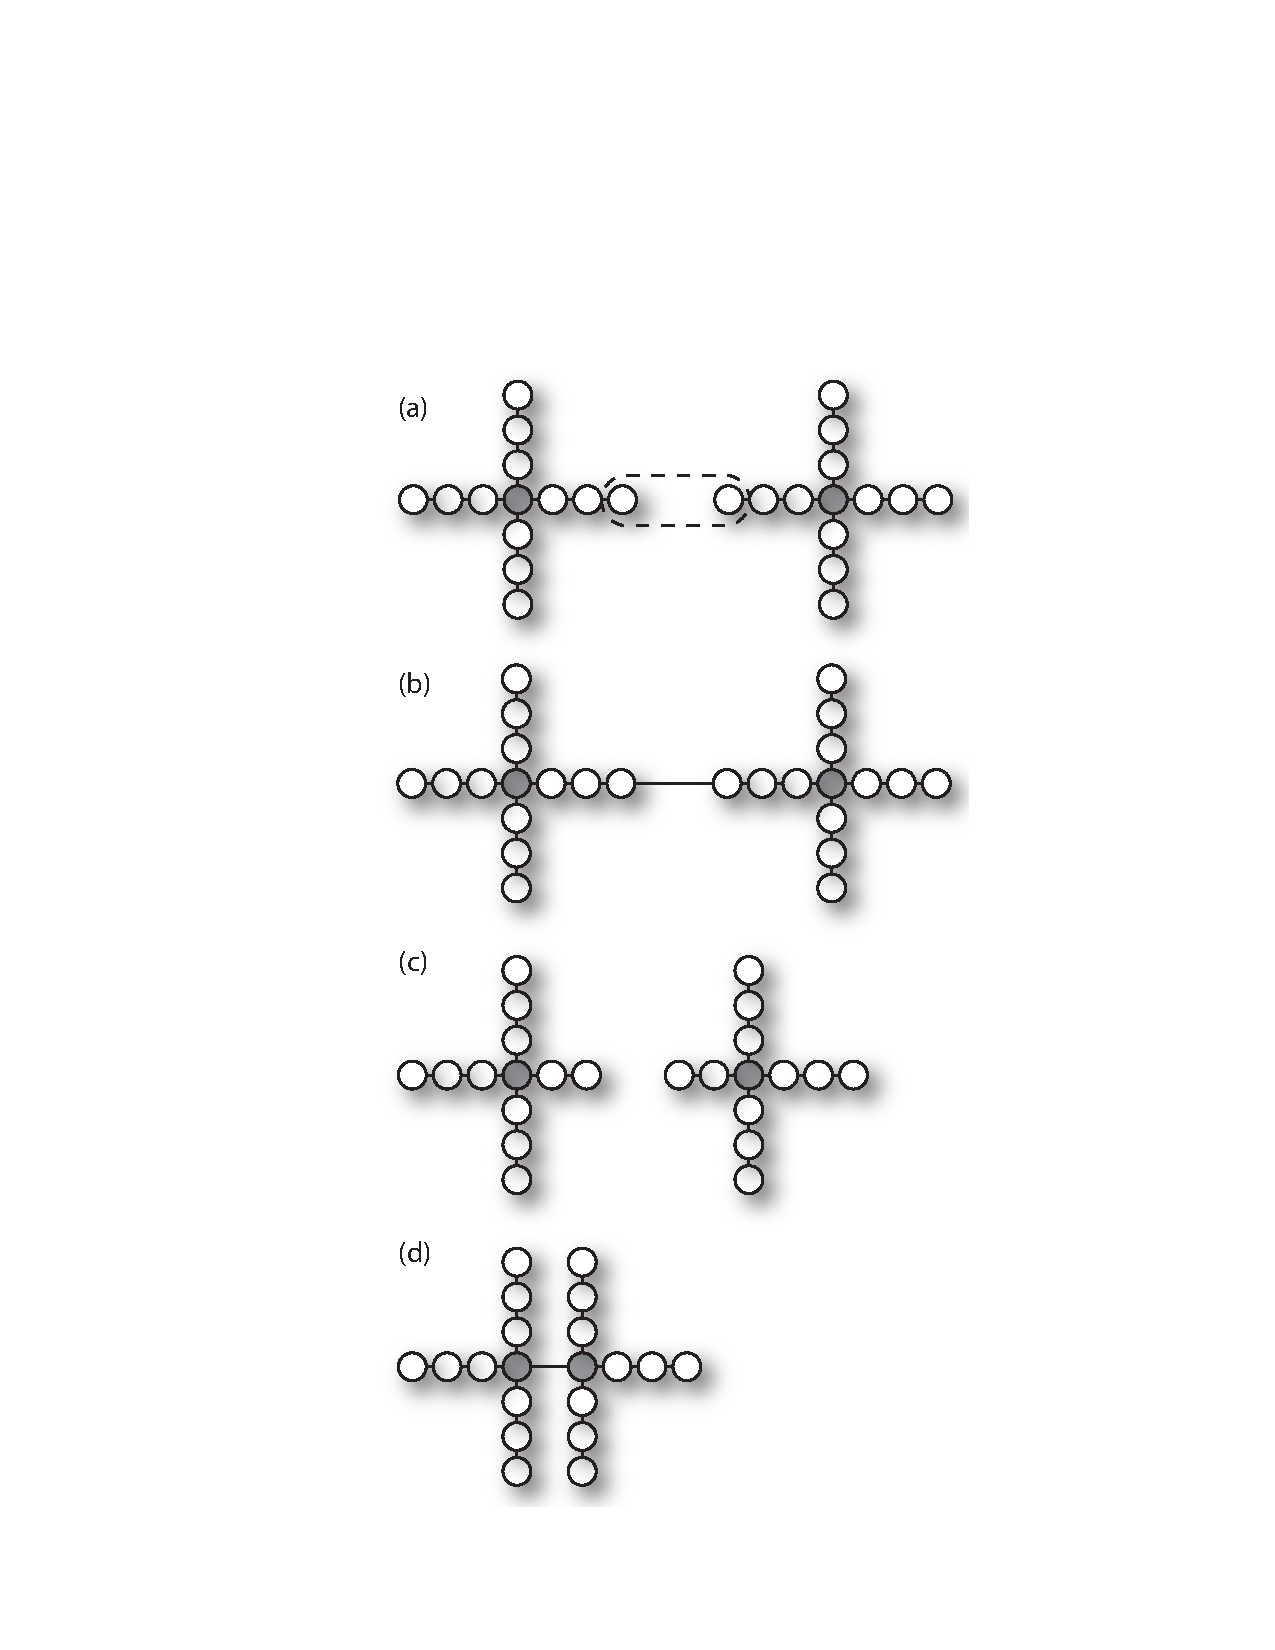
\includegraphics[clip=true, width=\textwidth]{cluster_ident}
	\captionspacefig \caption{Several cluster state identities for modularised quantum computation. (a) Two cluster states with a $+$-topology are fused together using an EO (dashed). (b) Upon success, an edge is created between the respective qubits. (c) Upon failure, both qubits are effectively measured in the $\hat{Z}$ basis, thereby removing them, and any associated edges, from the graph. (d) Following a successful EO, the unwanted ancillary qubits may be eliminated using measurements in the $\hat{Y}$ basis, creating edges between their neighbours. If the grey qubits represent the desired logical qubits, this can be used to remove the remainder of the branches emanating from them, thereby distilling the irregular graph down to a regular lattice.} \label{fig:plus_cluster_ident}
	\end{figure*}
\fi

We arrange the modules to internally represent a $+$-topology where each node has neighbouring branches in each of the up/down/left/right directions. But we imagine the situation whereby each logical qubit, along with its respective ancillary branches, is held by a different server. Thus, the final cluster state is truly decentralised across all the servers, and in general entire computations cannot be performed locally.

Using the ancillary states in the respective directions, we attempt to fuse neighbouring clusters using EOs, such as CZ gates (e.g a KLM CZ gate), linear optics \textit{fusion gates} (i.e rotated polarising beamsplitters followed by photo-detection, implementing which-path erasure\index{Which-path erasure}) \cite{bib:BrowneRudolph05}, or atoms with a $\lambda$-configuration coupled to photons \cite{bib:BarrettKok05}, which undergo which-path erasure (Sec.~\ref{sec:hybrid}). Importantly, using the fusion gate and which-path erasure approaches, only a single beamsplitter is required to perform the EO, which only necessitates high-visibility HOM interference, mitigating the need for far more challenging interferometric (MZ) stability (Sec.~\ref{sec:opt_stab}). This is delightful, as current leading quantum optics experiments routinely achieve HOM visibilities well in excess of 99\%.

An alternate fusion strategy is not to directly communicate qubits to be bonded, but instead rely off Bell pairs provided by a central authority. Each party then applies an EO between their half of the Bell pair and their target module qubit, which swaps the Bell pair entanglement onto the two respective module qubits (Sec.~\ref{sec:swapping}).

When an EO is successful, we have fused two modules together, albeit potentially with some leftover ancillary states between the logical qubits. When it fails, we have lost the respective ancillary states, and we attempt again using the next ancillary qubits in each of the the respective branches -- a kind of \textsc{Repeat Until Success} strategy. The bonding only fails if all $n_\mathrm{ancilla}$ EOs fail.

Note, however, that longer ancillary arms provide more opportunity for errors to accumulate \cite{bib:RohdeRalphMunro07}. Thus, despite its tolerance against gate failure, it is nonetheless highly desirable for EOs to be as deterministic as possible, so as to minimise the required number of ancillary qubits.

Upon successful bonding, any remaining ancillary qubits between the respective logical qubits are measured in the $\hat{Y}$ basis to remove them from the graph, whilst connecting their neighbours, leaving the two respective logical qubits as nearest neighbours in the graph. Now each module contains exactly one logical qubit, connected as desired to neighbouring modules. The relevant identities are shown in Fig.~\ref{fig:plus_cluster_ident}. Our goal is for the entire graph to have a lattice structure, once ancillary qubits have been measured out, as illustrated in Fig.~\ref{fig:module}.

\if 2\pubmode
\begin{figure}[!htbp]
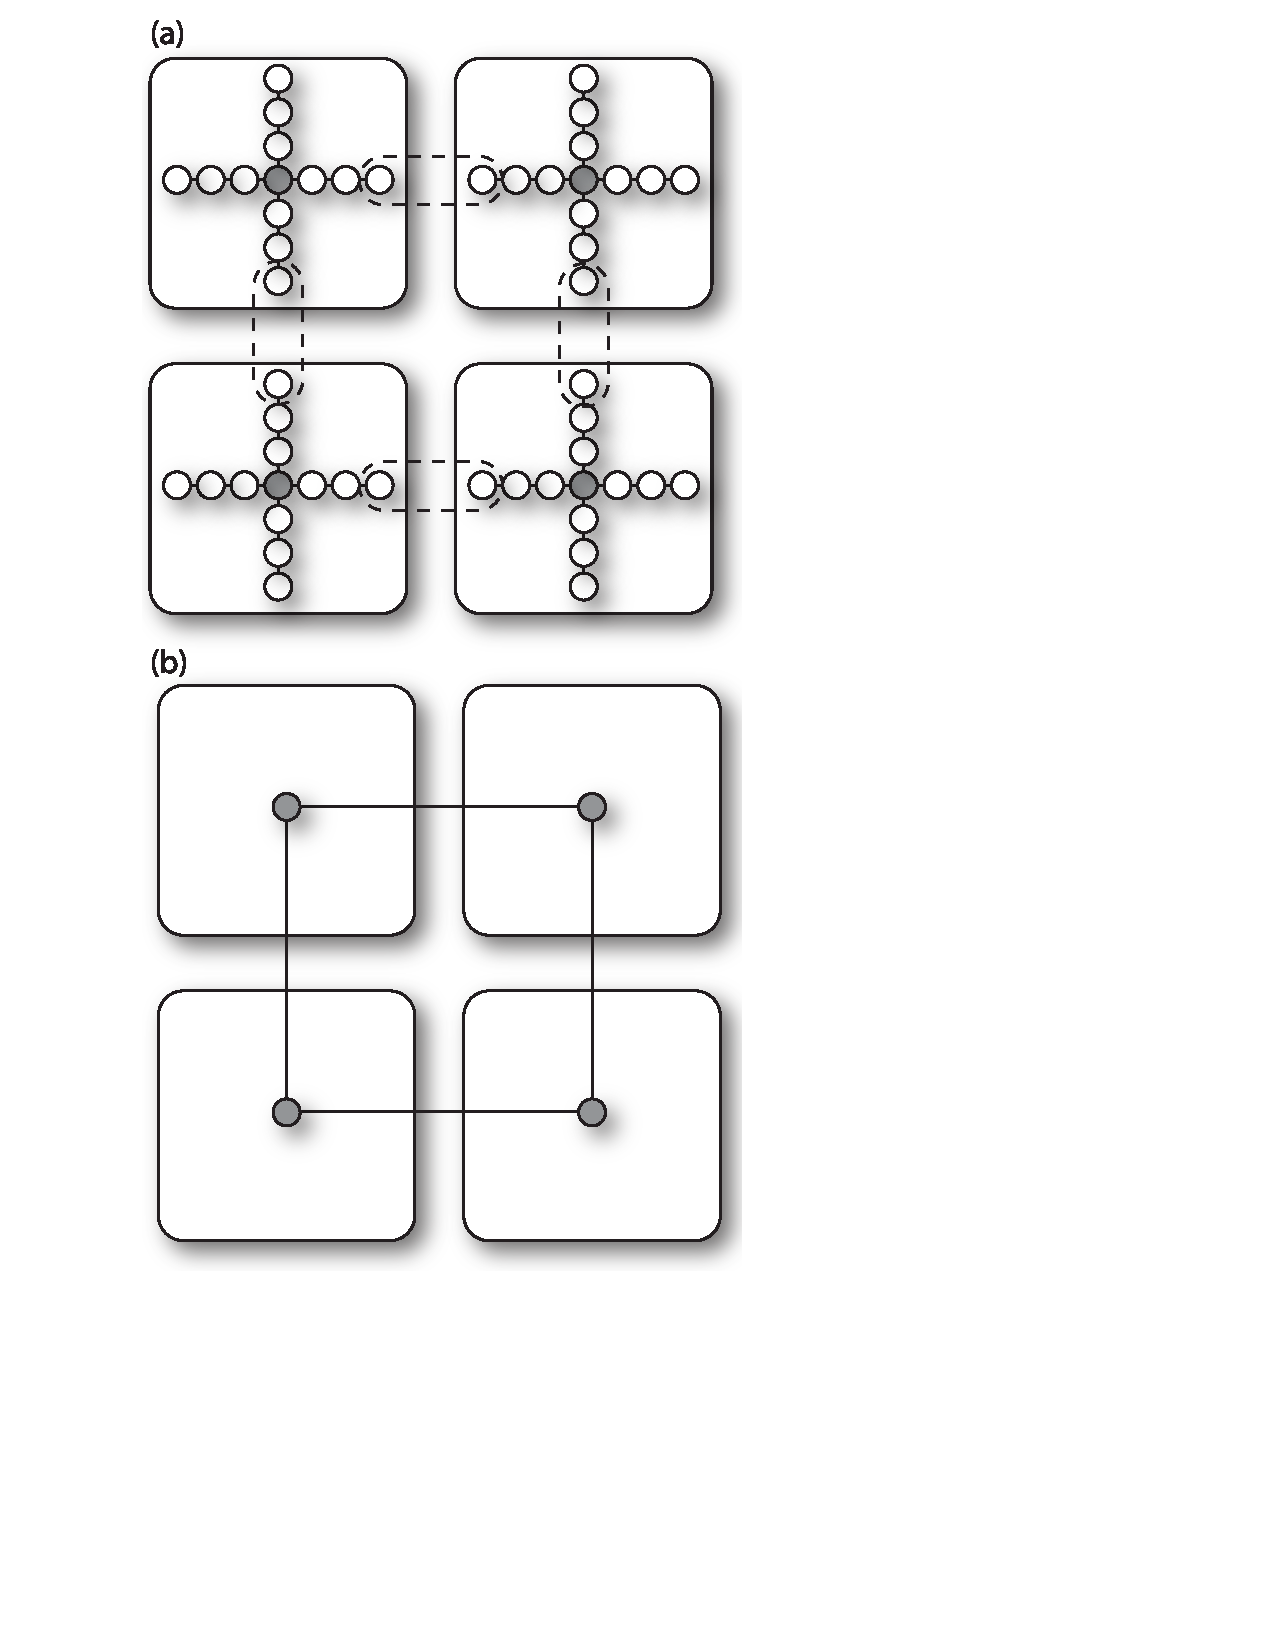
\includegraphics[clip=true, width=0.35\textwidth]{module_long}
\captionspacefig \caption{The modularised approach to scalable and economically efficient, distributed quantum computation using cluster states. The modules are all identical, and can be arbitrarily patched to one another, allowing the construction of arbitrary graph topologies. Because the modules are all identical, one might hope that mass production and economy of scale will drive down the cost of modules. We consider a simple \mbox{$2\times 2$} case where each module (rounded rectangles) comprises a single logical qubit (centre of each module in grey) and a number of ancillary qubits (white in each module), which facilitate bonding the logical qubits of nearest neighbours. The preparation of the modules is performed via nearest neighbour EOs (dashed ellipses), beginning at the end of branches, and working towards the root node upon each failure, until (hopefully) an EO is successful. (a) A \mbox{$2\times 2$} lattice of modules with their respective ancillary qubits. We attempt to bond the endpoints of chains using EOs. (b) Upon measuring the remaining ancillary qubits in the $\hat{Y}$ basis, only the logical qubits remain, with nearest neighbour bonds between adjacent modules, creating a distributed cluster state.} \label{fig:module}
\end{figure}
\else
\begin{figure*}[!htbp]
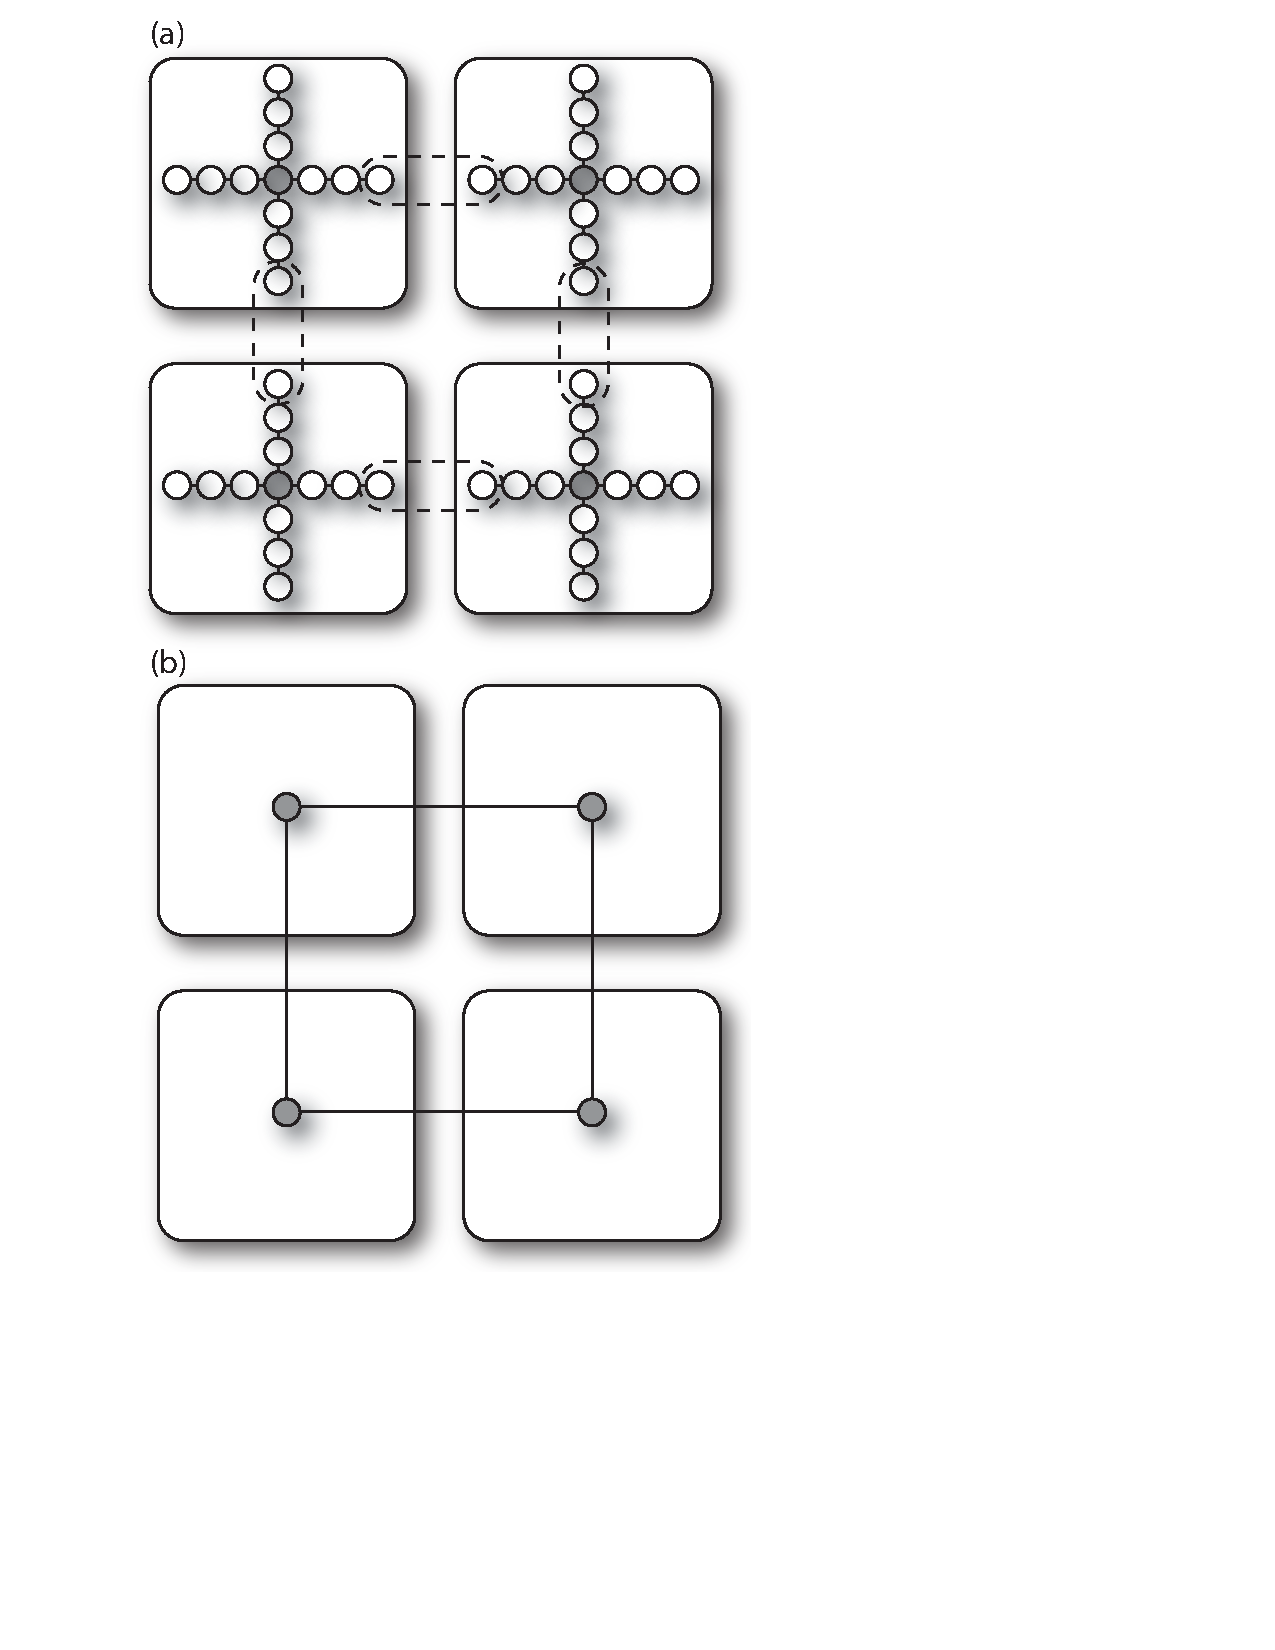
\includegraphics[clip=true, width=\textwidth]{module}
\captionspacefig \caption{The modularised approach to scalable and economically efficient, distributed quantum computation using cluster states. The modules are all identical, and can be arbitrarily patched to one another, allowing the construction of arbitrary graph topologies. Because the modules are all identical, one might hope that mass production and economy of scale will drive down the cost of modules. We consider a simple \mbox{$2\times 2$} case where each module (rounded rectangles) comprises a single logical qubit (centre of each module in grey) and a number of ancillary qubits (white in each module), which facilitate bonding the logical qubits of nearest neighbours. The preparation of the modules is performed via nearest neighbour EOs (dashed ellipses), beginning at the end of branches, and working towards the root node upon each failure, until (hopefully) an EO is successful. (a) A \mbox{$2\times 2$} lattice of modules with their respective ancillary qubits. We attempt to bond the endpoints of chains using EOs. (b) Upon measuring the remaining ancillary qubits in the $\hat{Y}$ basis, only the logical qubits remain, with nearest neighbour bonds between adjacent modules, creating a distributed cluster state.} \label{fig:module}
\end{figure*}
\fi

This approach has been shown to be resource-efficient \cite{bib:YoranReznik03, bib:Nielsen04}. Let us perform a rudimentary analysis of the resource scaling of this type of approach. The probability of successfully creating an edge between two modules is,
\begin{align}
p_\mathrm{success} = 1 - {p_\mathrm{failure}}^{n_\mathrm{ancilla}},
\end{align}
where $p_\mathrm{success}$ is the probability of joining two modules, $p_\mathrm{failure}$ is the probability that a single EO fails, and $n_\mathrm{ancilla}$ is the number of ancillary qubits per chain. $p_\mathrm{success}$ can be made arbitrarily close to unity with sufficiently long ancillary chains, the required length of whom scales as,
\begin{align}
n_\mathrm{ancilla} = \frac{\log (1-p_\mathrm{success})}{\log (p_\mathrm{failure})}.
\end{align}

Now, for simplicity we will consider the preparation of linear cluster states, although these ideas can easily be extended to more complex topologies, such as 2D lattice graphs.

Let us assume we have a `primary' linear topology of modules, which we will incrementally attempt to `grow' by tacking on new modules to the end. When we do so, with probability $p_\mathrm{success}$ we grow the length of the primary by 1, otherwise we decrement it by 1. This proceeds as a random walk, with on average \mbox{$2p_\mathrm{success}-1$} new qubits added to the primary per time-step. Provided this number is positive, i.e \mbox{$p_\mathrm{success}>1/2$}, which can always be achieved with sufficient $n_\mathrm{ancilla}$, the length of the primary grows linearly over time, allowing efficient state preparation.

This is just a very primitive model for preparing linear cluster states, using an equally primitive \textsc{Incremental} strategy for constructing them using non-deterministic gates. As discussed in Sec.~\ref{sec:CSQC}, much further work has been performed on the resource scaling of efficiently preparing cluster states of different graph topologies using different non-deterministic bonding strategies.

Of course, we have used the most simple model for modules, where each accommodates a single logical qubit. In due course, we would expect commodity modules to become far more capable, and resource scaling to improve. We might envisage that each module houses a small square lattice of logical qubits, as shown in Fig.~\ref{fig:larger_module}, and the interconnects between them glue them together like a patchwork quilt.

\begin{figure}[!htbp]
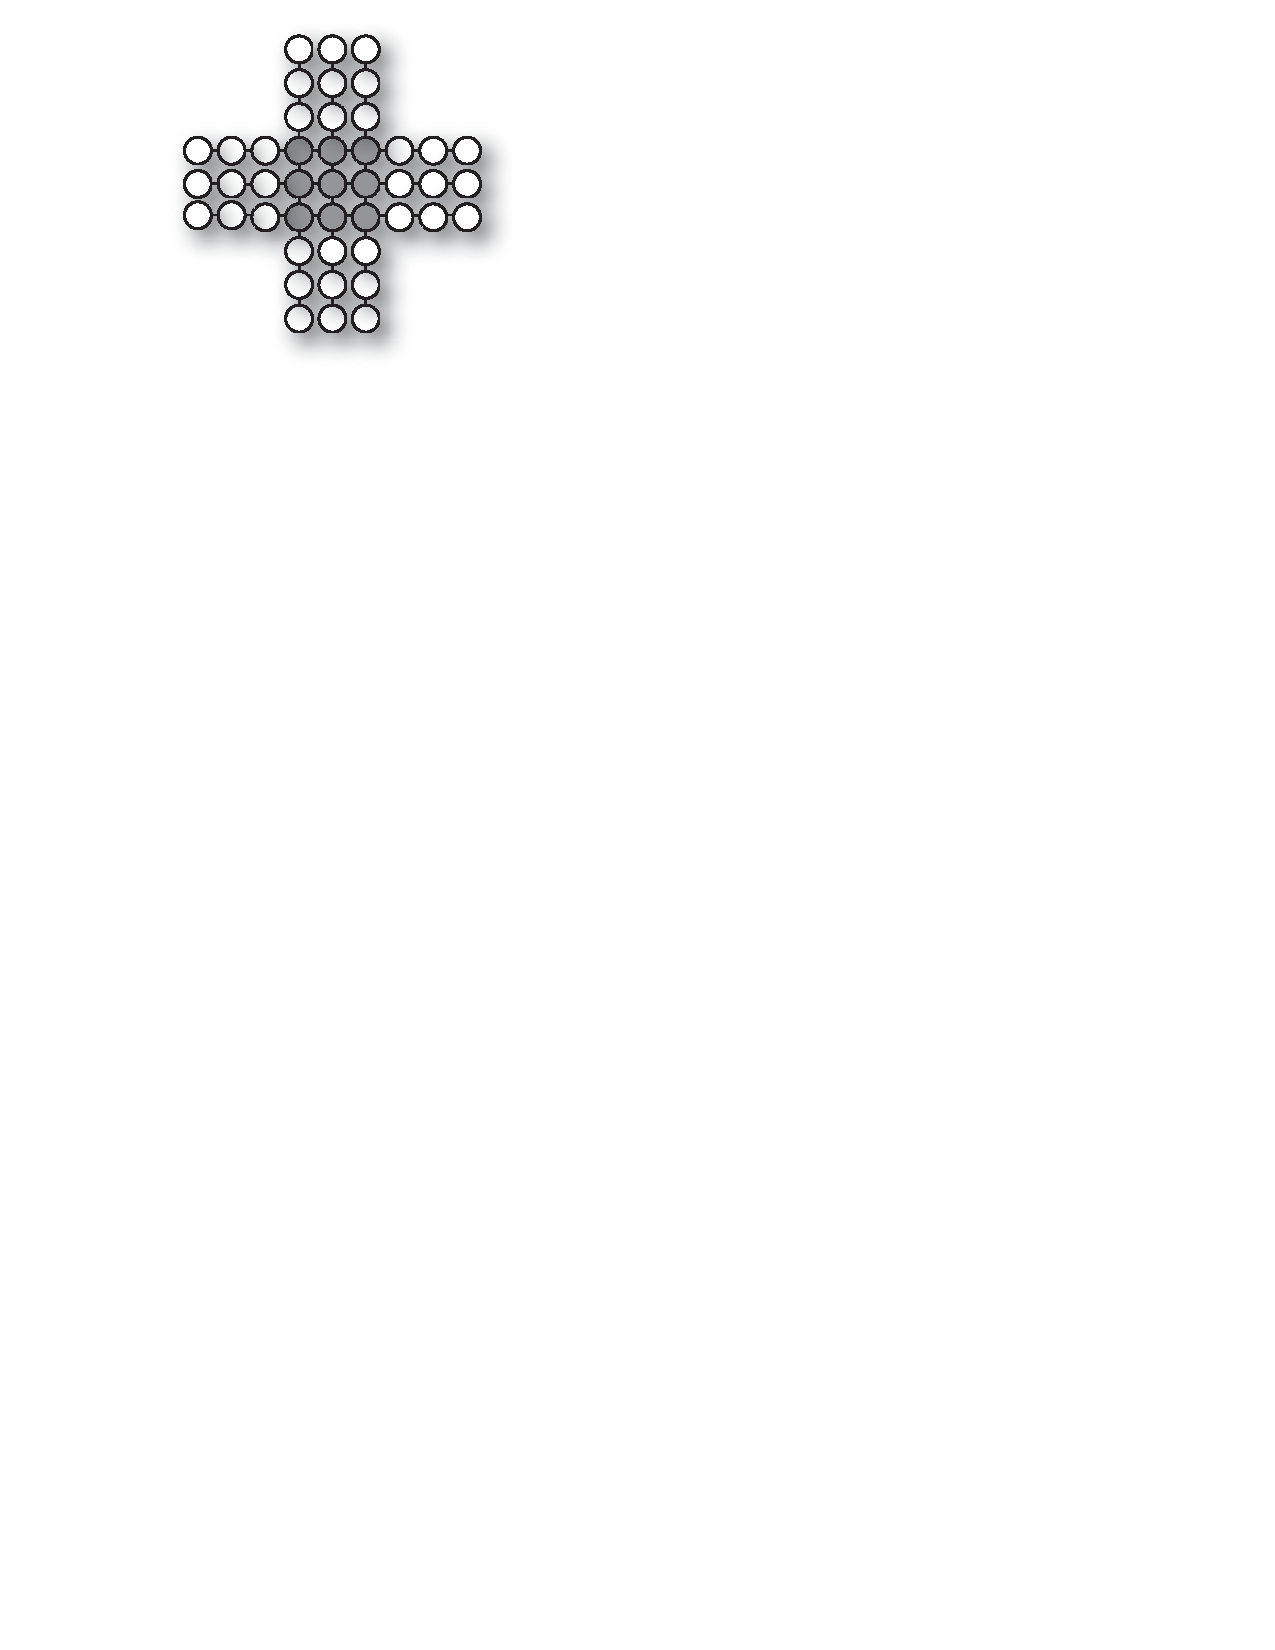
\includegraphics[clip=true, width=0.3\textwidth]{larger_module}
\captionspacefig \caption{A larger cluster state module comprising a \mbox{$3\times 3$} lattice of logical qubits (grey), and dangling arms of ancillary qubits (white) in each direction for joining them to neighbouring modules. Fusing these modules enables the `patchwork' preparation of large, distributed lattices.} \label{fig:larger_module}
\end{figure}

%
% Fundamental Physics Experiments
%

\subsection{Outsourced quantum research} \index{Outsourced!Quantum research}\index{Fundamental physics experiments}

Thus far we have focussed on computation as the key utility for outsourced quantum technologies, and certainly this is likely to be the dominant driving force behind quantum outsourcing\index{Outsourced!Quantum technology}. But of course not everyone wants to only solve complex algorithmic problems. Others may wish to study quantum systems themselves from the perspective of basic science research\index{Basic science research}, or perform precise quantum metrology.

It is foreseeable that in the context of a true quantum internet, there will be a demand for not only the communication of bits and qubits, but more general `quantum assets'\index{Quantum assets} (Secs.~\ref{sec:introduction} \& \ref{part:quant_net}), involving all manner of state preparation, manipulation, evolution and measurement, potentially all performed by different interconnected parties, specialising in different aspects of quantum protocols. The demand for this will extend far beyond computation.

The availability of a globe-spanning quantum satellite network brings the opportunity for fundamental quantum mechanical experiments and unprecedented length scales and velocities in the future. Satellite-to-satellite\index{Satellites!Satellite-to-satellite communication} photon transfer can allow for ultra-long distance quantum communications that are not possible on Earth due to atmospheric loss. Another unique aspect of space is that satellites move at high velocities -- typically at $10^{-5} $ times the speed of light\index{Speed of light} for LEO satellites. The combination of both of these effects gives a unique opportunity for performing relativistic quantum information\index{Relativistic quantum information} experiments to test fundamental physics. 

We anticipate that some of the first experiments will be extensions of what are already performed on Earth. For example, one can perform increasingly long space-based Bell violation tests\index{Bell!Inequality} at unprecedented distances \cite{bib:yin2017satellite}. Another possibility is to examine the speed of influence of entanglement \cite{bib:yin2013lower}. In space, such experiments could be extended much further, giving tighter bounds. There are demanding technical hurdles that must be overcome to succeed at such experiments, such as the necessity for synchronised clocks (Sec.~\ref{sec:clock_sync}).

 In addition to examining extensions of existing experiments, the high satellite velocities can be used to perform relativistic quantum information experiments, such as entanglement tests in the presence of special\index{Special relativity} and general relativity\index{General relativity}, Wheeler's delayed choice experiment\index{Wheeler's delayed choice experiment}, and enhanced quantum metrology \cite{bib:kaltenbaek2003proof, bib:scheidl2013quantum, bib:ahmadi2014relativistic}.

The QTCP protocol presented in Sec.~\ref{sec:QTCP} provides an extensible framework for facilitating these kinds of outsourced or delegated protocols\index{Outsourced!Protocols}\index{Delegated!Protocols} using generic quantum assets. Bear in mind that, as designed, the payload of QTCP packets could encapsulate all manner of optical states, or mediate long-distance interaction between them.

This model for quantum research could be invaluable to less-well-resourced researchers, for example in developing nations or not-so-well-funded universities, opening up a field of experimental research previously inaccessible to them. Indeed, some private and university sector operators are making elementary, remotely programmable quantum information processing protocols available over the internet, bringing this type of research within reach of researchers and even curious hobbyists around the globe.

While such early implementations fall far short of being truly reconfigurable, outsourced or delegated quantum protocols, applicable to a broad range of applications, they certainly already demonstrate the interest such models for outsourcing is generating within the research community, and the viability of further extending it.

Examples of how this type of model might be applied could include, but not be limited to research into:
\begin{itemize}
	\item Quantum information processing protocols, beyond only quantum computation, bits and qubits.
	\item Bose-Einstein condensates (BECs)\index{Bose-Einstein condensates (BECs)}.
	\item Light-matter interactions.\index{Light-matter!Interactions}
	\item Quantum thermodynamics and quantum statistical mechanics.\index{Quantum thermodynamics}\index{Quantum statistical mechanics}
	\item Quantum phase-transitions.\index{Quantum phase-transitions}
	\item Quantum optics, involving all manner of quantum states of light, beyond only those raised in Sec.~\ref{sec:opt_enc_of_qi}.\index{Quantum optics}
	\item Optical interferometry.\index{Optical!Interferometry}
	\item Providing a practical platform for university teaching and education.
\end{itemize}

In some instances, such outsourced quantum protocols might be applicable to encryption protocols, like those discussed in the next section (Sec.~\ref{sec:homo_blind}), enabling highly valuable secrecy for the experiments being conducted by researchers and their hard-earned results and ideas\footnote{Note, however, that the upcoming protocols are designed for application to particular optical states and protocols, and encryption schemes involving more generic quantum assets are likely to require some rethinking and adaptation (if possible at all, which isn't guaranteed!).}.

%
% The Globally Unified Quantum Cloud
%

\subsection{The globally unified quantum cloud}\index{Globally unified quantum cloud}\label{sec:glob_unif_quant_cloud}

In Sec.~\ref{sec:economics} we argue that in the quantum era it will be optimal to unify the world's quantum computers into a single virtual, distributed device, rather than utilising smaller individual quantum computers in isolation. This owes to the super-linear scaling in the power of a quantum computer against its number of constituent qubits, a phenomena unique to quantum computers with no classical parallel.

This economic imperative implies that the world's many clients of quantum computing will all be interacting will a single vendor -- the globally unified quantum cloud. This will create a competitive online marketplace for the licensing of timeshares in the utilisation of the unified device.

How this unified device will be managed, and by whom, is entirely open to speculation. Will a nation state or alliance of nation states monopolise it? Will a global consortium voluntarily emerge to manage the resources? Or will the whole thing be completely anarchic, potentially resulting in the fracturing of the unified device into several competing smaller ones? What policy and regulatory frameworks will emerge to oversee it? 

The answers to these questions are entirely uncertain. But what is certain is that there will be an extremely high level of unification of quantum resources via the quantum internet, massively enhancing its collective computational power.

The Quantum Cloud\texttrademark\, will be far more powerful than simply licensing compute-time from a single vendor. Its collective power will be far greater than the sum of its parts.